\documentclass[12pt, a4paper]{article}
\usepackage{graphicx}
\usepackage{xurl}
\usepackage{geometry}
\usepackage{float}
\usepackage{indentfirst}
\usepackage{amsmath}
\geometry{left=2.54cm, right=2.54cm, top=3.18cm, bottom=3.18cm}
% \setlength{\parindent}{0pt}

\title{Weekly Reports of Feedback Control RNN}
\author{Jerry Jin}

\begin{document}

\maketitle

\section*{Week 03/29 - 04/12}

\subsection*{Main Points}

\noindent
\begin{itemize}
    \item I get a deeper understanding of the hebbian correlation rule on readout matrix.
    \item I invent a kind of hebbian learning to solve the phase-shifting problem.
    \item I implement the framework of feedback control to replace the SGD on gains.

\end{itemize}

\newpage

\subsection*{Hebbian Correlation Rule on Readout Matrix}

The goal of feedback control is to make the output as the target (step 1). Then, hebbian learning could tune the readout weights accordingly (step 2). So it is possible to test hebbian learning separately: we could pretend the output is the target, and test where the hebbian learning would converge (see last week's "The Pipeline of Exploration").

However, this week I found that, \textbf{the hebbian correlation rule would always lead the readout weights to converge to the same point, no matter what the output is}.

First, let's recap our RNN:
$$x(t+1) = f(x(t), u(t), I(t))$$
where $x$ is the activation vector (1000 nodes), $u$ is the control input vector, $I$ is the input vector, $f$ is non-linear since there is the sigmoid activation function inside. In more detail:
$$x(t+1) = (1-c)*x(t) + c*\sigma((g+u(t)) * (Wx(t) + I(t) - s))$$
where $c$ is the time constant, $\sigma$ is the sigmoid activation function, $g$ is the gain vector, $u$ is applied on the gain (gain modulation), $W$ is the recurrent weight matrix, $s$ is the shift vector.

Now we're testing the convergence point of hebbian learning, so we are not giving the network any control input. So the network looks like this:
$$x(t+1) = (1-c)*x(t) + c*\sigma(g * (Wx(t) + I(t) - s))$$

For now, the input to every node is $I_i(t) = a_i \sin(\frac{\pi}{60}t)$, the sine wave multiplied by a random weight. Then, spontaneously, the activation of every node would converge to a sine wave with the same frequency but different phases and amplitudes.

\begin{figure}[H]
    \centering
    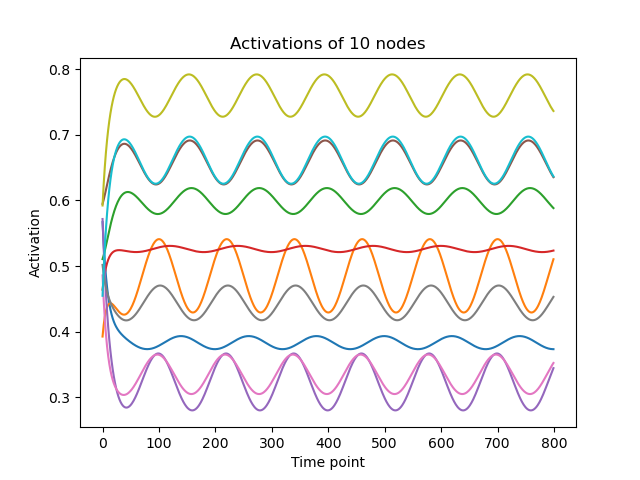
\includegraphics[width=0.8\textwidth]{RNN/FORCE/fig/FORCE_ff_activations.png}
\end{figure}

The output is $z(t)=\sigma(g_{out}*(Hx(t)-s_{out}))$, where $H$ is the readout matrix, $g_{out}$ is the gain of the output node, $s_{out}$ is the shift of the output node. At this stage, although everything is just initialized and I did not tune anything, \textbf{the output is already a sine wave} (with a random scale), since it is just a weighed sum of sine-like activations.

Now, if I turn the hebbian learning on, the readout weights would converge to a point where \textbf{each weight is proportional to the mean activation of the corresponding node} (see the second figure in last week's "Deepen the Understanding of Last Week's Result"). This is because, at each step of the hebbian learning, we are doing $h_i \leftarrow h_i + x_i z$ and then doing the normalization (keeping the sum of $h_i$ as constant), so the $H$ would finally converge to a point proportional to the mean of $x(t)$.

So finally, after the hebbian learning, the output would be a sine wave with a certain scale. I could just hand-tune the $g_{out}$ and $s_{out}$ (or use some very simple algorithm, since there is just 2 parameters) to make the scale the same as the target sine wave. Finally, we would get a phase-shifted target sine wave (see the first figure in last week's "Deepen the Understanding of Last Week's Result").

In summary, to get a phase-shifted target sine wave is really a simple process. We only need to input a sine wave with the same frequency, then every node in the network would follow a sine wave with that frequency. The output is a weighed sum of every node, and Hebbian learning is just changing the way of doing the weighed sum (in the way that the readout weights are proportional to the mean activations).

\newpage

\subsection*{A Hebbian Learning Rule that Correct the Phase}

From the last section, we know that the hebbian correlation rule would lead the weight of one node to be proportional to the mean activation of that node. It could not help the output to have a correct phase as the target. So we'll always get a phase-shifted sine wave. Is there a way to use hebbian learning to learn the correct phase? I invented a hebbian learning rule based on the hebbian correlation rule: $$h_i \leftarrow h_i + (z(t) - \bar{z}) \frac{x_i(t) - \bar{x_i}}{\text{std}(x_i)}$$
You can image $\bar{x_i}$ and $\text{std}(x_i)$ as constant. If $x_i(t)$ and $z(t)$ has very different phase (e.g., one is at peak while the other one is at trough), then $h_i$ would always decrease. If $x_i(t)$ and $z(t)$ has the same phase, then $h_i$ would increase. (Of course, there is the Dale's law, so for excitatory nodes $h_i$ can't be below zero and for inhibitory nodes $h_i$ can't be above zero; and there is a following normalization to prevent increasing or decreasing infinitely.)

To plot out the relative shift of phase of each node's activation to the target and the readout weights after this hebbian learning, we could get a curve with peak at 0 and a trough at 60 (since here the input and the target sine wave have a period of 120). 

\begin{figure}[H]
    \centering
    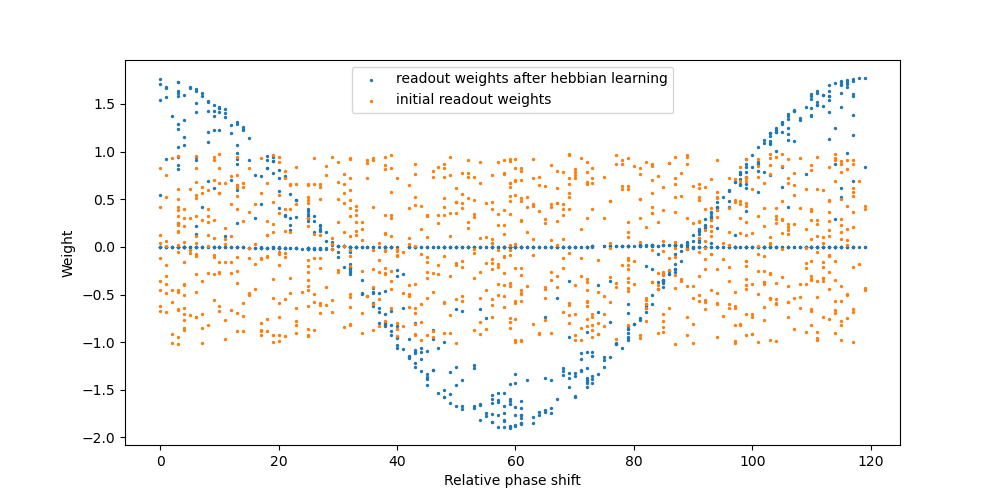
\includegraphics[width=\textwidth]{RNN/FORCE/fig/FORCE_phase_outweights.png}
\end{figure}

The last step would be to divide the readout weight of each node by the mean activation of that node (so that each node contribute equally to the phase of the output). Then, we could get a output with the correct phase as the target (here the target is $\sin(\frac{\pi}{60}(t+20))$.

\begin{figure}[H]
    \centering
    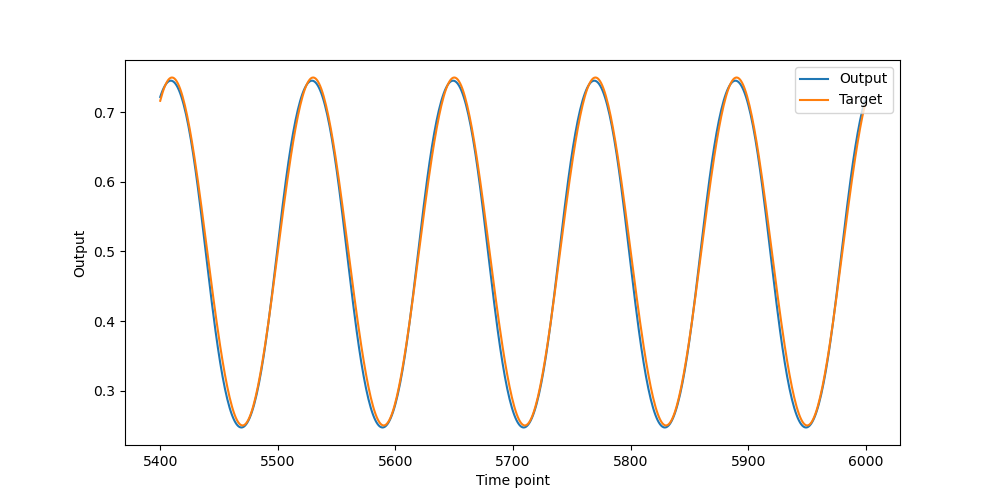
\includegraphics[width=\textwidth]{RNN/FORCE/fig/FORCE_phase_output.png}
\end{figure}

Note: in this section we're still testing hebbian learning, so we pretend that $z(t)$ is the target while doing hebbian learning. Also, to get a uniform distribution of relative shift of phase across nodes, the input to each node is a sine wave with a random phase, $I_i(t) = a_i \sin(\frac{\pi}{60}(t+t_i))$. 

In summary, in this section we achieve the result that inputing each node with a sine wave with fixed frequency but random phase, we could use hebbian learning to make the output follows a sine wave with an arbitrary phase.

\newpage

\subsection*{LQR Feeback Control for RNN}

Following last week, I applied the discrete-time optimal control for tracking a desired output. Let our target be $\tilde{z}(t)$, then an ideal trajectory for $Hx(t)$ is $\tilde{y}(t) = \text{inverse\_sigmoid}(\tilde{z}(t))$. 

Applying quadratic control, it is to minimizing the loss $$V = \sum_{t=t_0+1}^T (y(t) - \tilde{y}(t))^T Q_2 (y(t)- \tilde{y}(t)) + u(t-1)^T R u(t-1)$$

In fact, the idea is to generalize the $V$ to $$V = \sum_{t=t_0+1}^T \bar{y}(t)^T Q_1 \bar{y}(t) + (y(t) - \tilde{y}(t))^T Q_2 (y(t)- \tilde{y}(t)) + u(t-1)^T R u(t-1)$$ where $\bar{y} = \bar{H}y = (I - H^T(HH^{T})^{-1}H)y$

It is equivalent to calculate a desired state $\tilde{x}(t) = H^T(HH^{T})^{-1}\tilde{y}(t)$ and so $$V = \sum_{t=t_0+1}^T (x(t) - \tilde{x}(t))^T Q (x(t)- \tilde{x}(t)) + u(t-1)^T R u(t-1)$$ where $Q=\bar{H}^T Q_1 \bar{H} + H^T Q_2 H$

We set $Q_1 = 0.1I$, $Q_2 = 10I$, $R=0.0001I$, and use Jacobian matrix to do the linear approximation of the non-linear system. We could get a result like following, where the control seems not bad:

\begin{figure}[H]
    \centering
    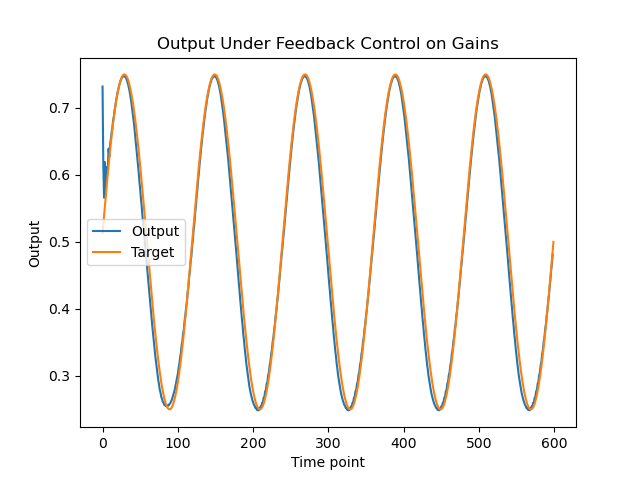
\includegraphics[width=0.8\textwidth]{RNN/FORCE/fig/FORCE_tracking_output_0412.png} \\
\end{figure}

Next steps: connect the feedback control framework with the hebbian learning; try a set of basis functions as input (what is an example?).

\newpage

\section*{Week 03/15 - 03/29}

\subsection*{Goal}

\noindent
\begin{itemize}
    \item Try to merge the hebbian learning of readout matrix into the framework of feedback control, instead of using SGD.
    \item Try to input a set of basis functions, instead of inputing only the target.

\end{itemize}

\newpage

\subsection*{The Pipeline for Exploration}

To my understanding, we want our network to do the following steps:

\begin{enumerate}
    \item The network initializes with initial gains, initial shifts, intial weights.
    \item With feedback control, we modulate the gains and shifts so that the network outputs the target.
    \item Keeping the output as the target, Hebbian learning modifies the weights and returns gains and shifts to their initial values. Thus, the network could finally output the target with initial gains, initial shifts, and modified weights. 
\end{enumerate}

I had several attempts where step 2 is successful but step 3 is not. A common issue is that the gains and shifts refuse to return to their initial values after Hebbian learning is turned on. Another common issue is that the weights could not converge.

A successful step 3 implies that there must exist a \textbf{convergence point} for weights under Hebbian learning, where the network could output the target with initial gains and shifts.

So I come up with an idea to test step 3 separately. We "pretend" that step 2 is done perfectly and that the network is outputing the target. We do Hebbian learning using the target. (Normally, $w_{i} \rightarrow w_{i} + \eta r_i z$, where $r_i$ is the activation of node $i$ and $z$ is the activation of the output node, but now we use the target as $z$, pretending that the output node is activated correctly.) With initial gains, initial shifts, and such Hebbian learning, we could test whether the weights could converge to an convergence point where the actual output is closed to the target.

If such test is passed, once step 2 is successful and the output is clamped to the target, Hebbian learning would drive weights to that convergence point, so that step 3 is acheived.

\newpage

\subsection*{Deepen the Understanding of Last Week's Result}

Recall that last week I gave the network the target sine wave as input and trained the readout matrix. After going through step 1 to 3, the network finally produces a phase-shifted sine-wave. 

To find out why there was this phase-shifting problem, I did the test of step 3 described above (i.e., using the target as pretended output to perform the Hebbian learning). I found that the network naturally converge to a point where the actual output is the phase-shifted sine wave.

\begin{figure}[H]
    \centering
    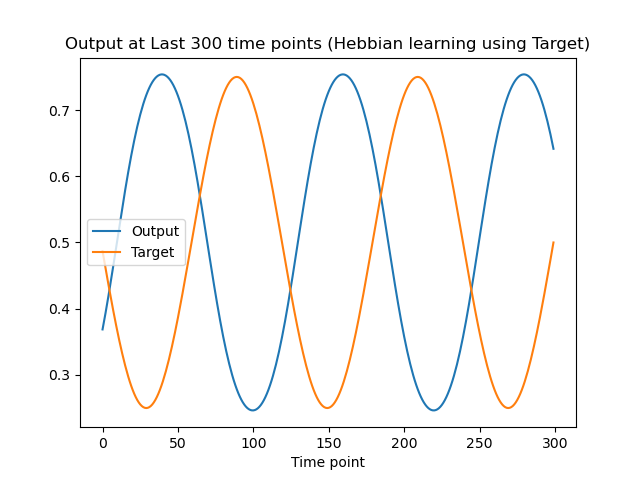
\includegraphics[width=0.8\textwidth]{RNN/FORCE/fig/FORCE_targethebb_lastoutput.png} \\
\end{figure}

Also, through observation, we could see that every node has a sine-like activation, with different phases. The output is the weighed sum of all those sine waves. Hebbian learning on the readout matrix is just to adjust these additive weights. However, a correlation Hebbian learning rule cares more about the average amplitude of each sine wave, rather than the phase. So I guess to solve the problem requires the Hebbian covariance rule.

\begin{figure}[H]
    \centering
    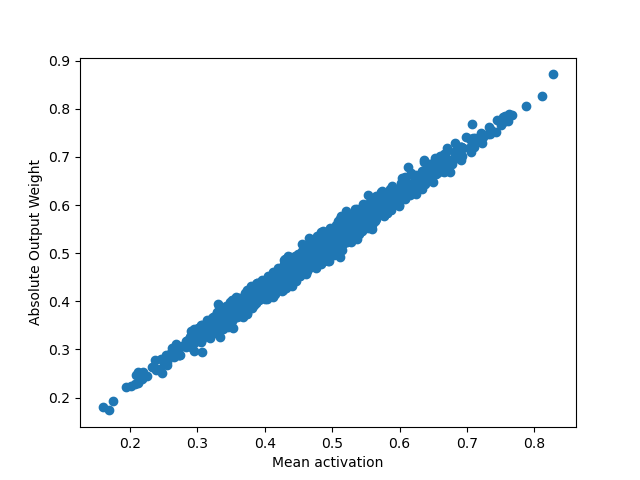
\includegraphics[width=0.8\textwidth]{RNN/FORCE/fig/FORCE_fbtargethebb_weightcorractv.png} \\
\end{figure}

\newpage

\subsection*{Input a Set of Basis Functions}

Since inputing the target to the network may not be ideal in realistic situation, we could change it to input a set of basis functions. Here, I try to input different sine waves with random frequency and phase to each node. Then the activation would look like this:

Again, I did the test of step 3 described above. The hope is that Hebbian learning could suppress those with wrong frequency and wrong phase and strengthen those with correct frequency and correct phase. Again, Hebbian correlation rule could not do this. With Hebbian covariance rule, a primitive result looks like this. I'm not sure whether it would work if I twist some details. Still need more attempts.

\begin{figure}[H]
    \centering
    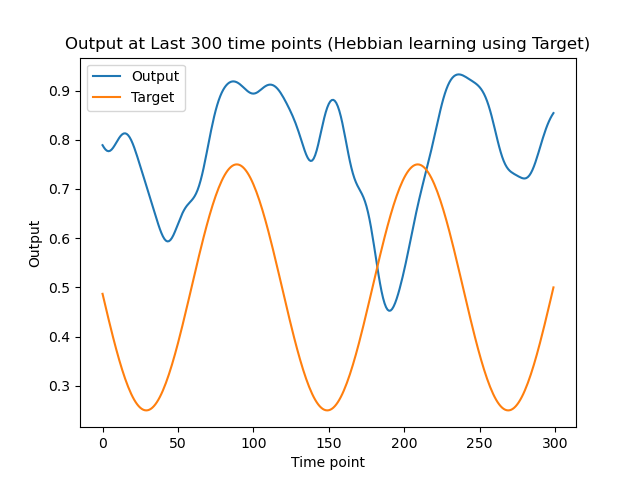
\includegraphics[width=0.8\textwidth]{RNN/FORCE/fig/FORCE_wavebasis_outputhcp.png} \\
\end{figure}


\newpage

\subsection*{Merge with The Feedback Control Structure}

The goal is to use control theory rather than SGD to achieve step 2, for the current RNN. Though I realized such stucture to correct perturbation, it turns out that there are more things to be done. Previously, I have a trained network which could produce ideal sine waves. Under perturbation, the idea is to drive the system state to \textbf{the desired state}. But where could we know the desired state? It is achieved a priori from runs without perturbation (admittedly, this is a little bit cheating). 

But here and in a more realistic situation, we would not know the desired state, but \textbf{the desired output}. After consulting Ankit, I learn that this would be a more complex control problem called tracking problem in control theory. And since our network has other inputs and our network is simulated in discrete time, the full name would be discrete-time model-following tracking problem. I am reading the textbook from Anderson and Moore (1989), and I am still working to get the things done properly. 

To formulate our control problem, we have a system: 
$$x(t+1) = f(x(t), u(t), I(t))$$
where $x$ is the activation, $u$ is the control input, $I$ is the input, $f$ is non-linear since there is the sigmoid activation function.

The output is:
$$y(t) = Hx(t), z(t) = \text{sigmoid}(y(t))$$
where $H$ is the readout matrix (output weight matrix). Our target is $\tilde{z}(t)$, which is a sine wave. Since sigmoid is monotonic, we could calculate an ideal trajectory for $Hx(t)$, denoted as $\tilde{y}(t) = \text{inverse\_sigmoid}(\tilde{z}(t))$.

Applying quadratic control, it is to minimizing the loss $$V = \sum_{t=t_0+1}^T (y(t) - \tilde{y}(t))^T Q (y(t)- \tilde{y}(t)) + u(t-1)^T R u(t-1)$$

We could use the linear approximation of our non-linear system and apply the linear quadratic control theory. Currently, the results look like this:

\begin{figure}[H]
    \centering
    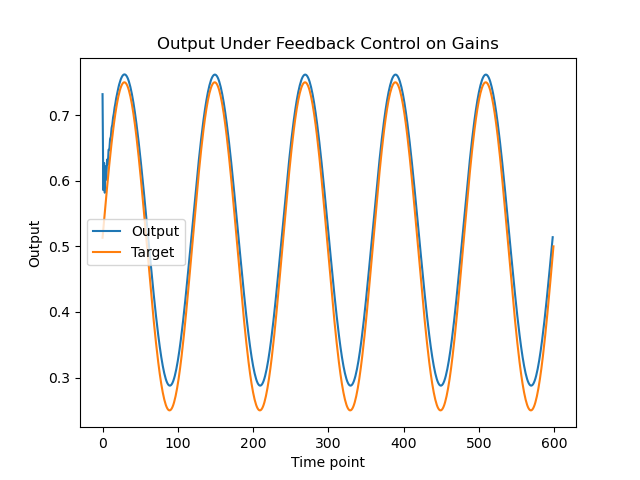
\includegraphics[width=0.8\textwidth]{RNN/FORCE/fig/FORCE_tracking_output.png} \\
\end{figure}

Since I feel like there are still problems, I did not proceed to try Hebbian learning (step 3). 

\newpage


\section*{Week 02/20 - 03/15}

\subsection*{Goal}

\noindent
\begin{itemize}
    \item Understand the hebbian learning in RNN.
    \item I try the idea of only modifying readout matrix in RNN (borrowing the idea FORCE learning).
    \item More systematic perturbation experiments in the feedforward network (changing amplitude).

\end{itemize}

\newpage

\subsection*{RNN with Gain Modulation and Hebbian Learning on Output Weight Matrix}

To understand RNN, I read the FORCE learning paper again (Sussillo \& Abbott, 2009) as well as a MIT tutorial on FORCE learning. They mentioned that, if there is a strong teaching signal for every nodes, the RNN would be much more stable, even if it has chaotic spontanueous activities. What's more, they used a Recursive Least Square algorithm to train only the readout matrix (that is, output weight matrix), leaving the N by N recurrent weight matrix intact. This procedure could let RNN to produce very complex patterns. So I decide to try the idea of only modifying output weight matrix. Instead of modifying it directly (e.g., Recursive Least Square), we could modifying the gains and shifts of each neurons first and then using Hebbian learning to modify the output weight matrix.

First, I start from an RNN without input. Its recurrent layer has N = 1000 neurons, half excitatory and half inhibitory, following Dale's law. $\mathbf{x}$ denotes the N-dimensional state vector of this layer before the activation function, and $J$ denotes the N by N recurrent weight matrix. So the RNN is simulating this equation:

$$\frac{d\mathbf{x}}{dt} = -\mathbf{x} + J f(\mathbf{x}) $$

All recurrent neurons connect to an output neuron through the output weight matrix $w$, giving the output $z$:

$$z = f_{out}(\mathbf{w}^T f(\mathbf{x}))$$

$f$ here represents the sigmoid activation function for each neuron, with adjustable gains and shifts. For this step, we initialize all gains as 1 and all gains as 0 for all recurrent neurons. For the output neuron $f_{output}$, the gain is 1.15 and the shift is -2.5 (hand-tuned).

The $J$ and $w$ I'm using are shown below.

\begin{figure}[H]
    \centering
    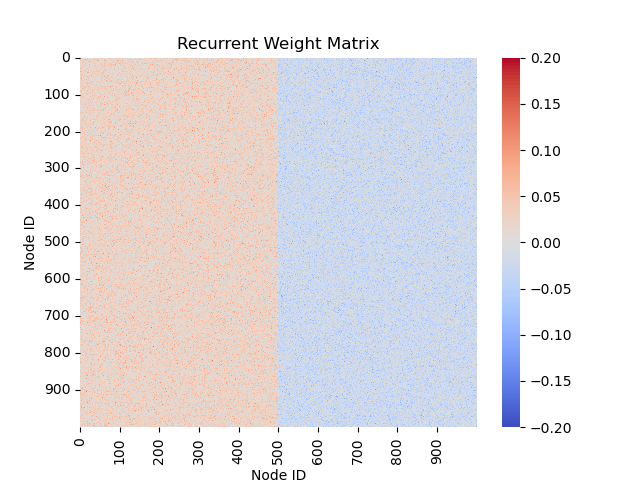
\includegraphics[width=0.6\textwidth]{RNN/FORCE/fig/FORCE_nofb_rcweight.png} \\
    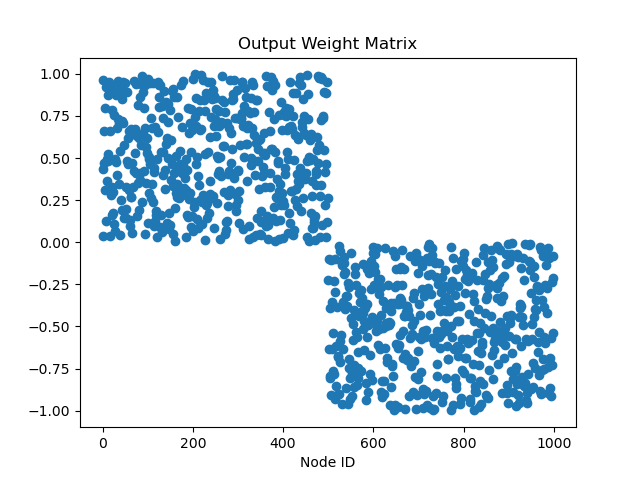
\includegraphics[width=0.6\textwidth]{RNN/FORCE/fig/FORCE_nofb_outweight.png} \\
\end{figure}

The RNN shows a convergence of activity for all neurons. (Note that I use quite the same parameters as Sussillo \& Abbott 2009, but I change their tanh activation function to sigmoid, and I applies Dale's law. Their network shows a chaotic activity.)

\begin{figure}[H]
    \centering
    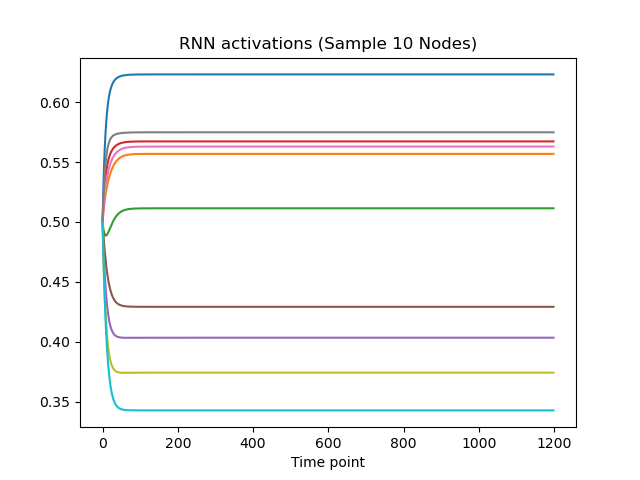
\includegraphics[width=0.6\textwidth]{RNN/FORCE/fig/FORCE_nofb_activations.png} \\
    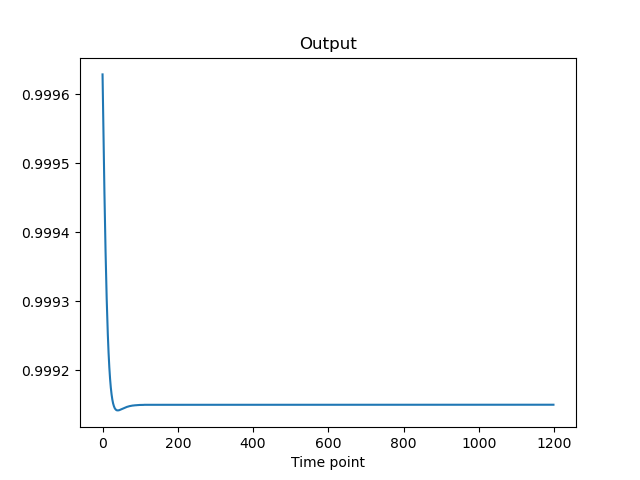
\includegraphics[width=0.6\textwidth]{RNN/FORCE/fig/FORCE_nofb_output.png} \\
\end{figure}

Second, I input the target signal $\sin(\omega t)$ to every neurons by some input weight matrix $u$. So now the RNN is simulating the following equation:

$$\frac{d\mathbf{x}}{dt} = -\mathbf{x} + J f(\mathbf{x}) + \sin (\omega t) \mathbf{u} $$

Now the RNN shows a periodic activity for all neurons.

\begin{figure}[H]
    \centering
    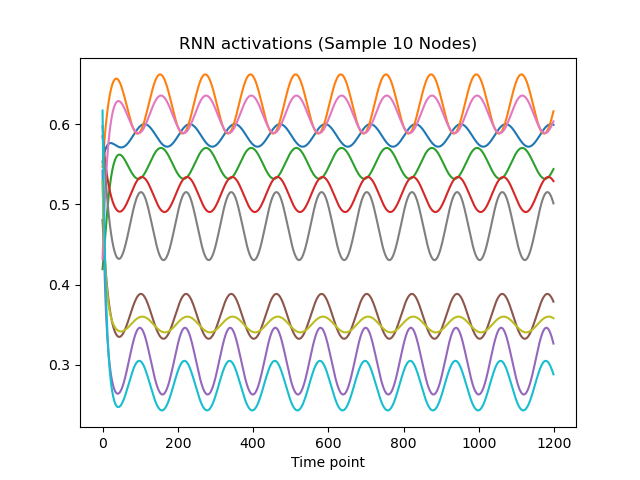
\includegraphics[width=0.6\textwidth]{RNN/FORCE/fig/FORCE_fbtarget_activations.png} \\
    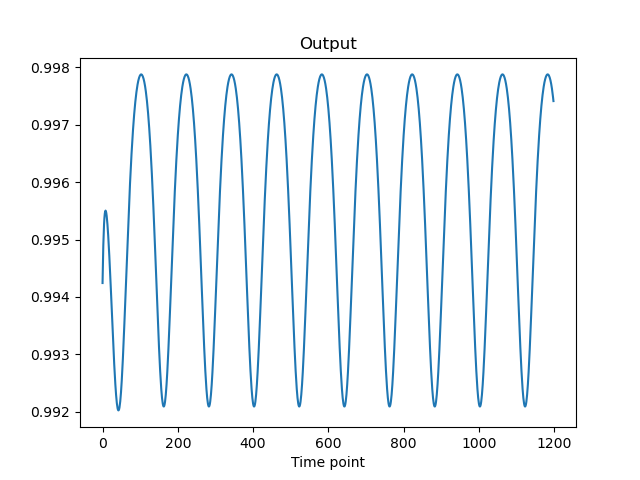
\includegraphics[width=0.6\textwidth]{RNN/FORCE/fig/FORCE_fbtarget_output.png} \\
\end{figure}

The third step is to add gain modulation and hebbian learning. I use SGD to update the gains and shifts of every neuron in the reccurrent layer after every period of sine wave, so that the output is closed to the target signal (the output neuron is intact all the time). Then, after the loss is small (800000 time points), I turn on the hebbian learning to modify the output weight matrix. The hebbian rule is a simple correlation rule, $w_{i} \rightarrow w_{i} + \text{Sign}(w_i) \eta f(\mathbf{x_i}) z$. So positive weights are always becoming more positive and negative weights are always becoming more negative. To prevent exploding, there is also a normalization step to keep the sum of all positive weights as 250 and the sum of all negative weights as -250.

We show that gain modulation could indeed make output close to the target.

\begin{figure}[H]
    \centering
    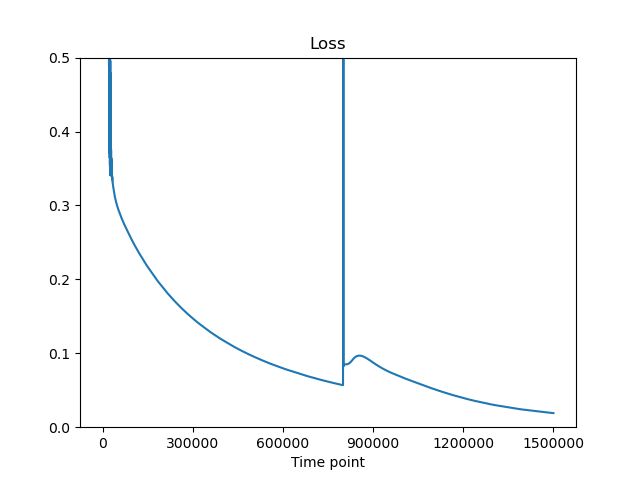
\includegraphics[width=0.6\textwidth]{RNN/FORCE/fig/FORCE_fbtargethebb_loss.png} \\
    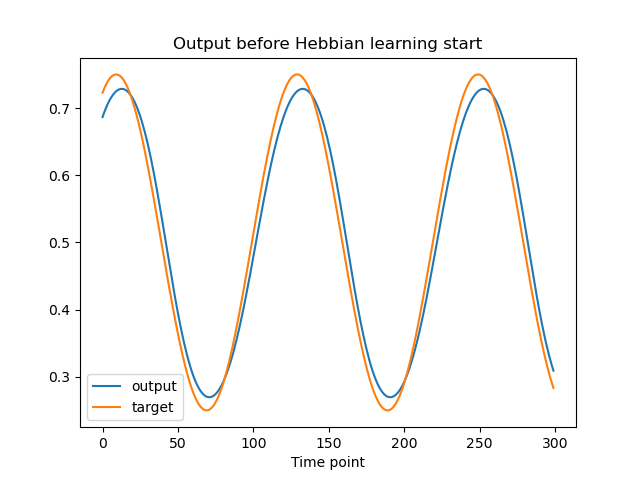
\includegraphics[width=0.6\textwidth]{RNN/FORCE/fig/FORCE_fbtargethebb_SGDoutput.png} \\
    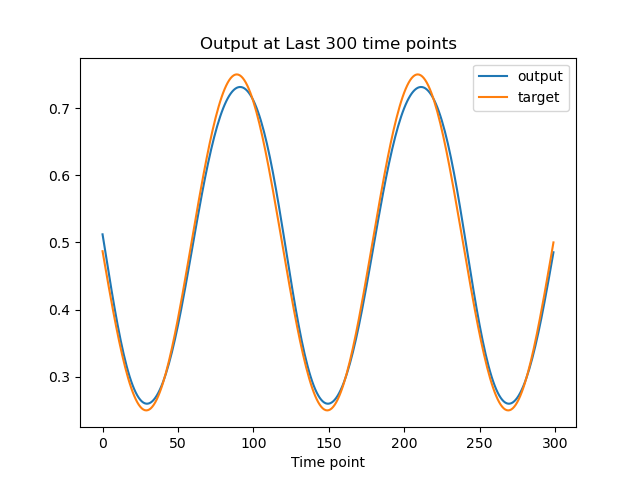
\includegraphics[width=0.6\textwidth]{RNN/FORCE/fig/FORCE_fbtargethebb_lastoutput.png} \\
\end{figure}

And the Hebbian learning does modify the output weight matrix.

\begin{figure}[H]
    \centering
    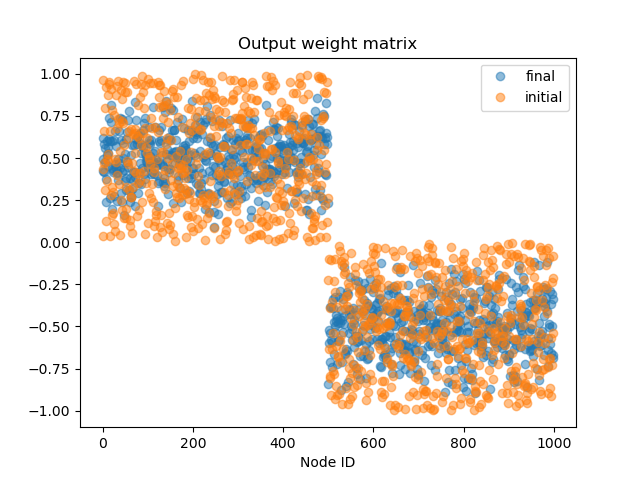
\includegraphics[width=0.6\textwidth]{RNN/FORCE/fig/FORCE_fbtargethebb_outweight.png} \\
\end{figure}

Although during the training the change in gains and shifts is ramping up continuously, amazingly, if I just use the inital gains and shifts after training, the network could simulate sine wave quite well, apart from some alignment problem and phase shifting problem.

\begin{figure}[H]
    \centering
    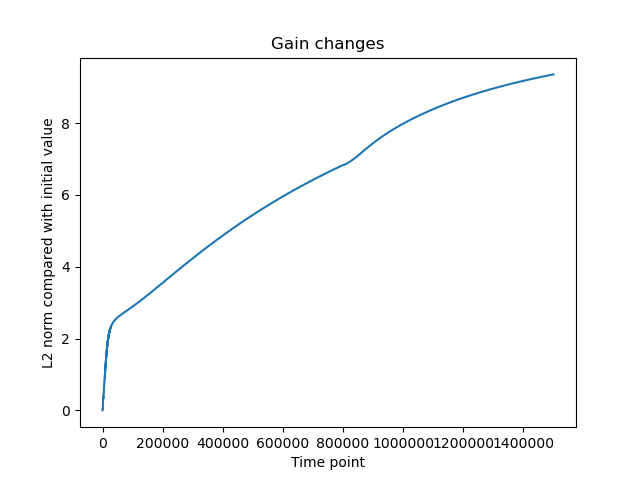
\includegraphics[width=0.6\textwidth]{RNN/FORCE/fig/FORCE_fbtargethebb_theogc.png} \\
    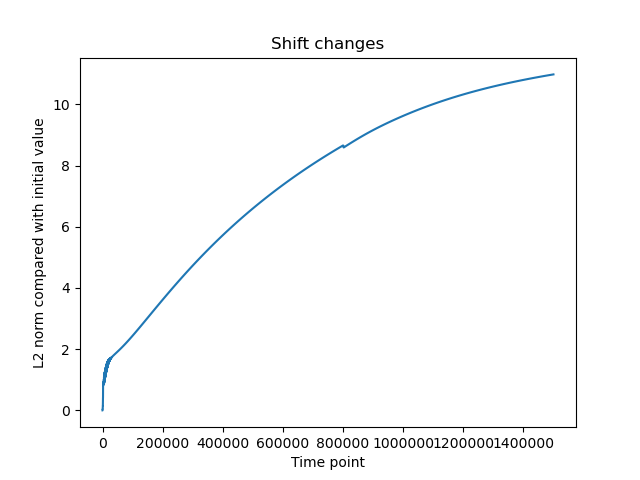
\includegraphics[width=0.6\textwidth]{RNN/FORCE/fig/FORCE_fbtargethebb_theosc.png} \\
    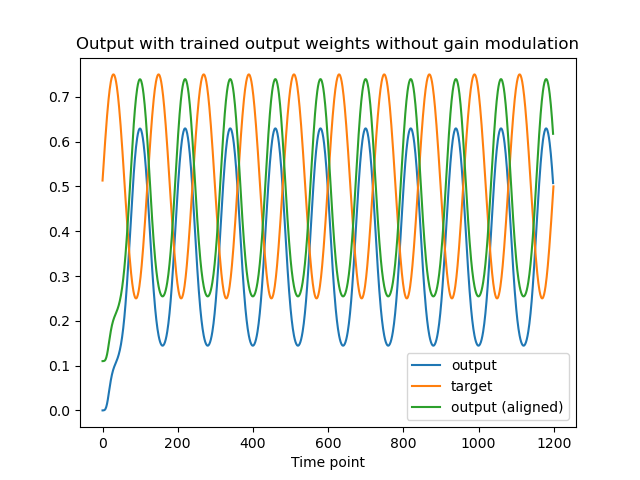
\includegraphics[width=0.6\textwidth]{RNN/FORCE/fig/FORCE_fbtargethebb_nogainoutput.png} \\
\end{figure}

The phase shifting problem is also a problem mentioned in Sussillo \& Abbott (2009). And I think it is because of phase shifting, the change of gains and shifts don't decrease during training. This is a problem need to be solve at next stage. Other potential improvement includes turning on hebbian learning gradually.

\newpage

\subsection*{Perturbation in Feedforward Network}

I found some more subtle details about perturbation experiments in feedforward network.

Firstly, there are two ways to add perturbation. One way is to add perturbation \textbf{inside the sigmoid activation function} ($r_i = \frac{1}{1 + e^{-g_i(I_i-s_i) + \epsilon_i}}$, where $\epsilon_i$ is the perturbation), another way is to add perturbation o\textbf{utside the sigmoid activation function} ($r_i = \frac{1}{1 + e^{-g_i(I_i-s_i)}} + \epsilon_i$). The former way would not change the range of $r_i$ (0 to 1), while the latter would change the range of $r_i$.

Secondly, for experimenting on perturbation lasting, we expect that a longer perturbation would result in more difficulties in recovery. We observe the expected effect when perturbation is \textbf{outside sigmoid} with amplitude = 0.1 (see previous week). But this is a fortunate case where convergence happens quickly during perturbation. In other cases, for example, when the perturbation is too weak or the perturbation is \textbf{inside sigmoid (as below)}, during perturbation convergence might take more epoches. And if you stop perturbation before convergence, the effect would not be so stable.

\begin{figure}[H]
    \centering
    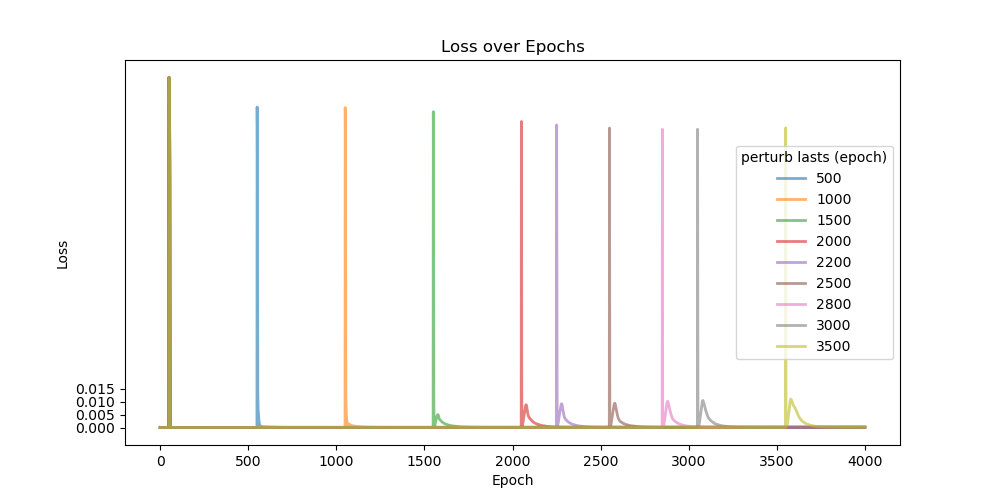
\includegraphics[width=0.9\textwidth]{FNN/fig/temp_abb05_perturb_loss_train_insigmoid.png} \\
    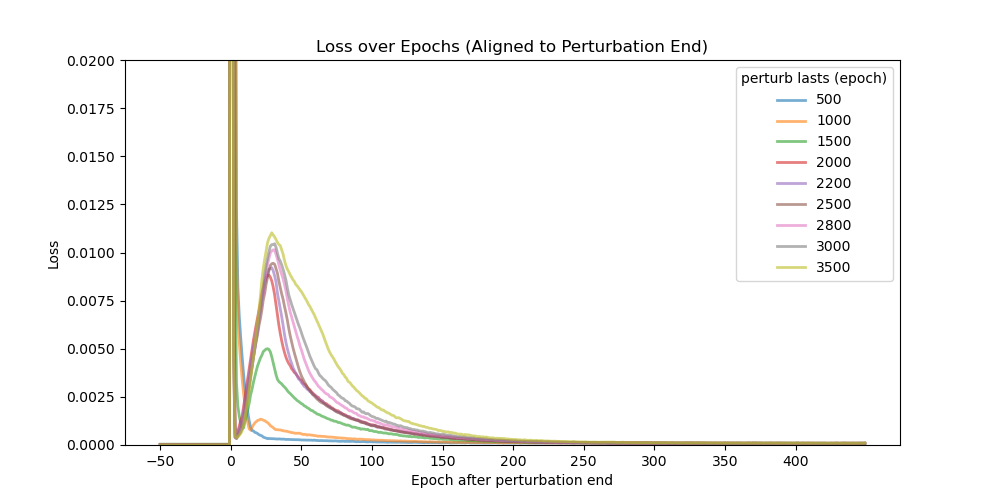
\includegraphics[width=0.9\textwidth]{FNN/fig/temp_abb05_perturb_loss_align_insigmoid.png} \\
\end{figure}

\begin{figure}[H]
    \centering
    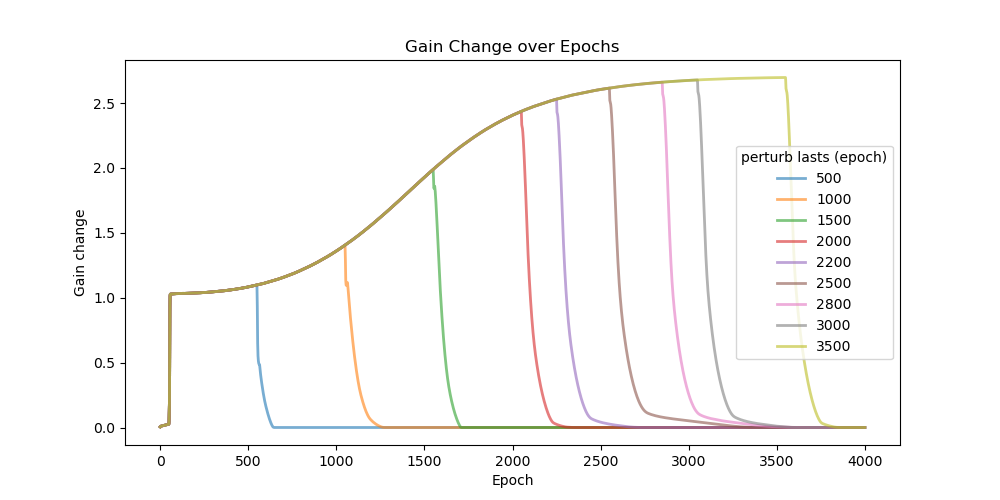
\includegraphics[width=0.9\textwidth]{FNN/fig/temp_abb05_perturb_gc_insigmoid.png} \\
    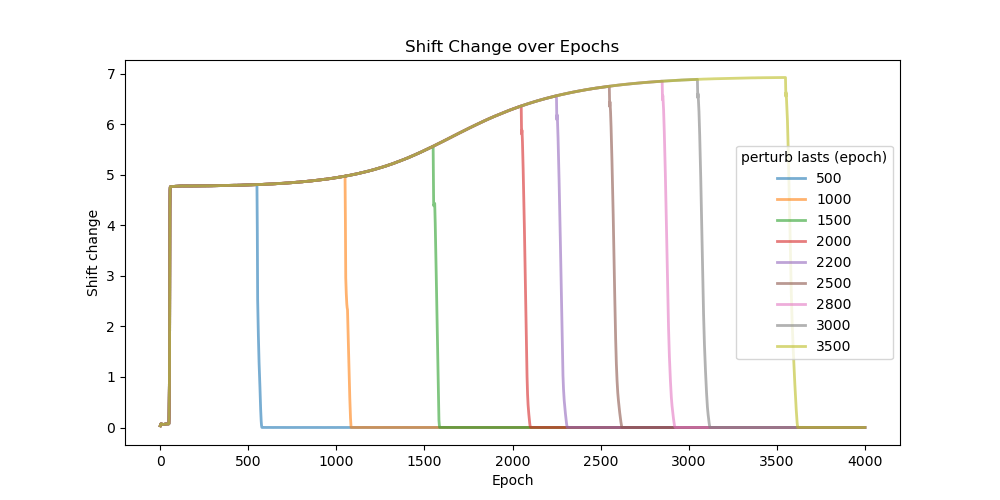
\includegraphics[width=0.9\textwidth]{FNN/fig/temp_abb05_perturb_sc_insigmoid.png} \\
\end{figure}


\begin{figure}[H]
    \centering
    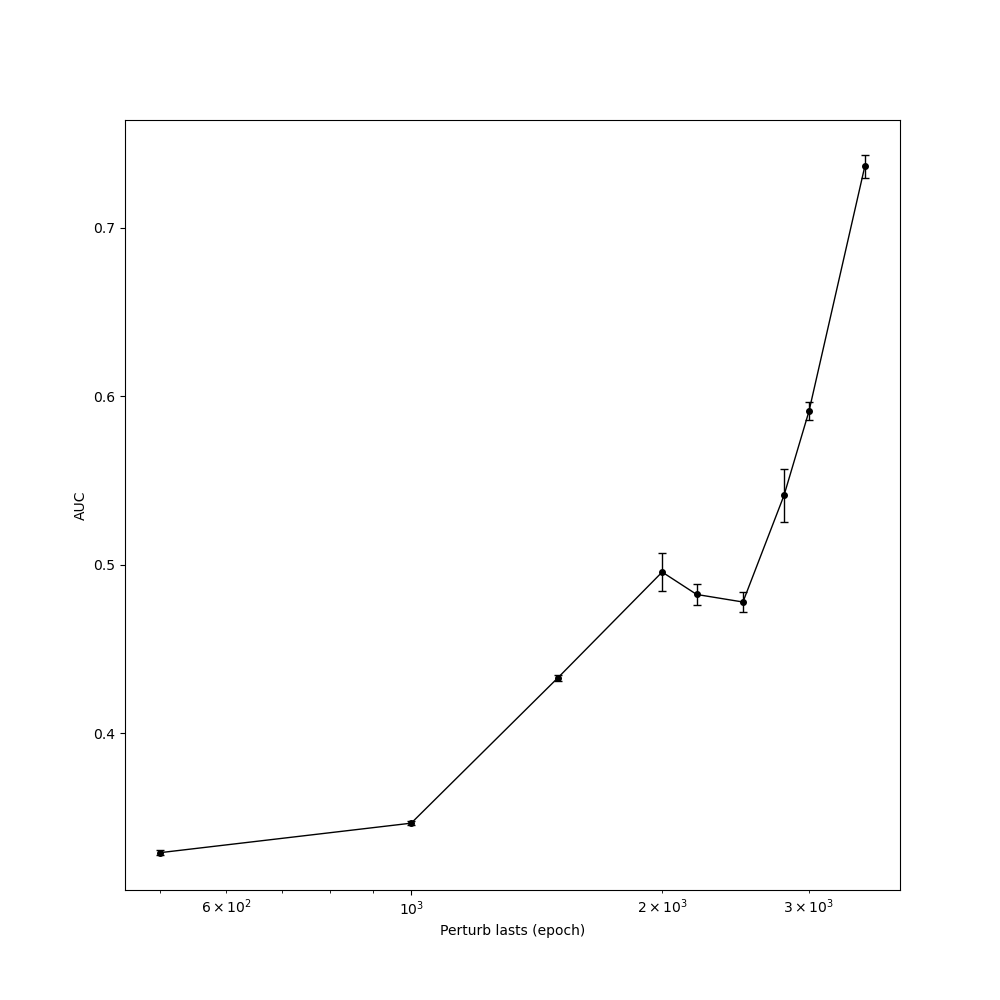
\includegraphics[width=0.6\textwidth]{FNN/fig/temp_abb05_perturb_auc_insigmoid.png} \\
    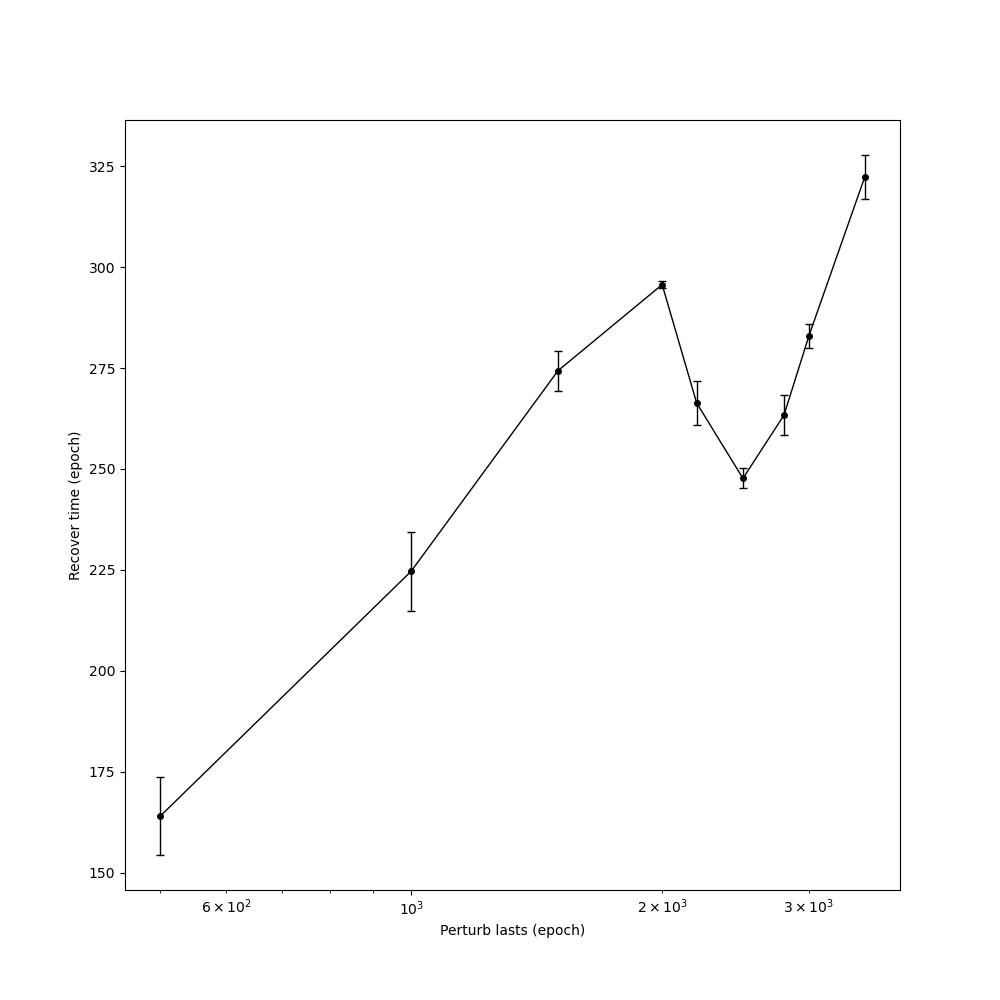
\includegraphics[width=0.6\textwidth]{FNN/fig/temp_abb05_perturb_rectime_insigmoid.png} \\
\end{figure}

Thirdly, for experimenting on perturbation amplitude, we expect that a too large perturbation would result in saturation in sigmoid, which in turn causes no learning during perturbation and the recovery would be quick. We observe the basic effect for perturbation \textbf{inside sigmoid} (see previous week). However, there are other cases where perturbation is outside sigmoid, or there is partial learning during perturbation, or recovery fails, to be explored (as below).

\begin{figure}[H]
    \centering
    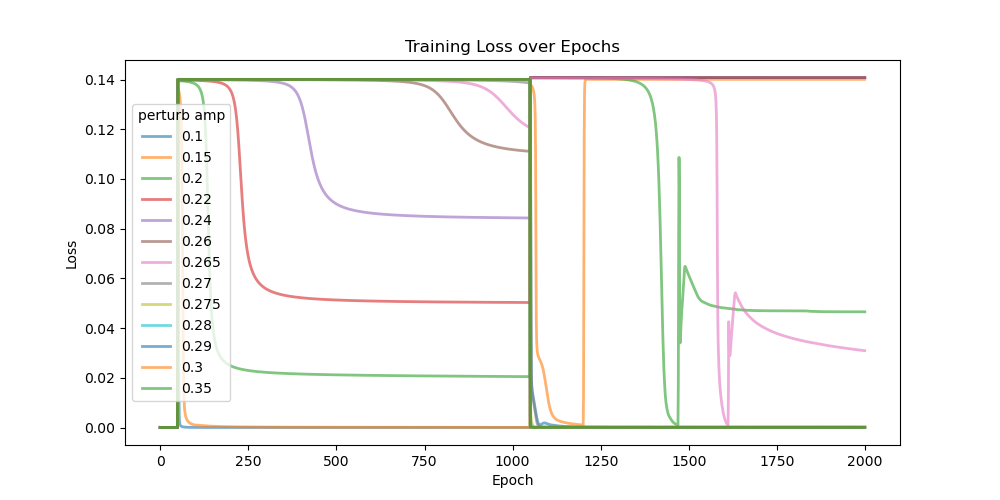
\includegraphics[width=0.9\textwidth]{FNN/fig/temp_abb05_perturbamp_loss_outsigmoid.png} \\
\end{figure}

\begin{figure}[H]
    \centering
    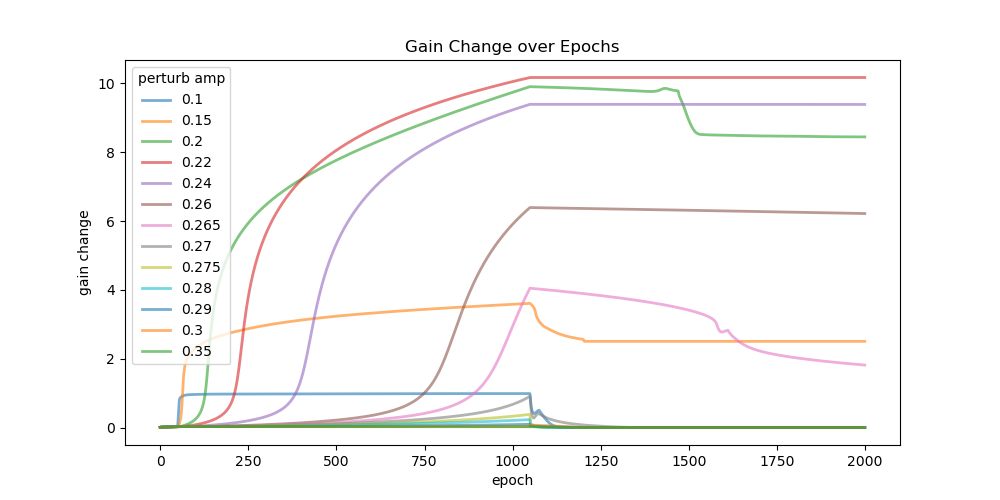
\includegraphics[width=0.9\textwidth]{FNN/fig/temp_abb05_perturbamp_gc_outsigmoid.png} \\
    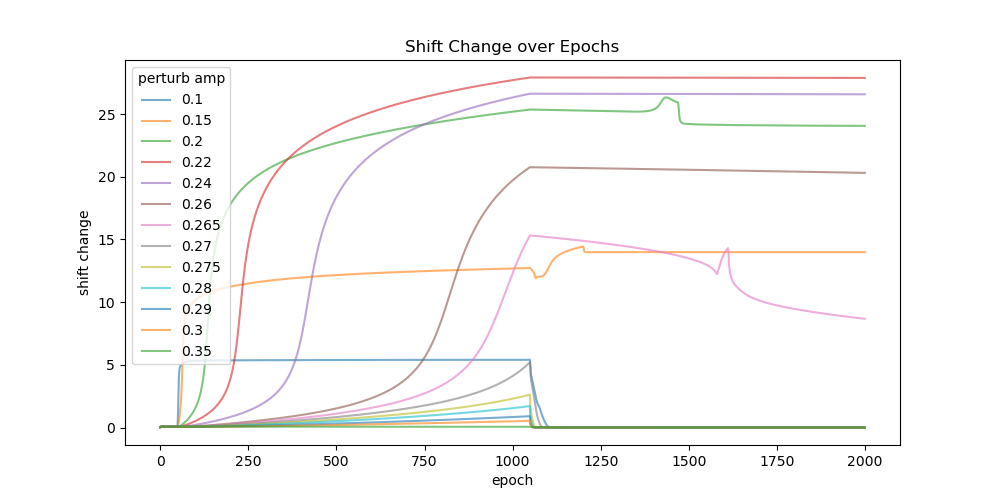
\includegraphics[width=0.9\textwidth]{FNN/fig/temp_abb05_perturbamp_sc_outsigmoid.png} \\
\end{figure}


\begin{figure}[H]
    \centering
    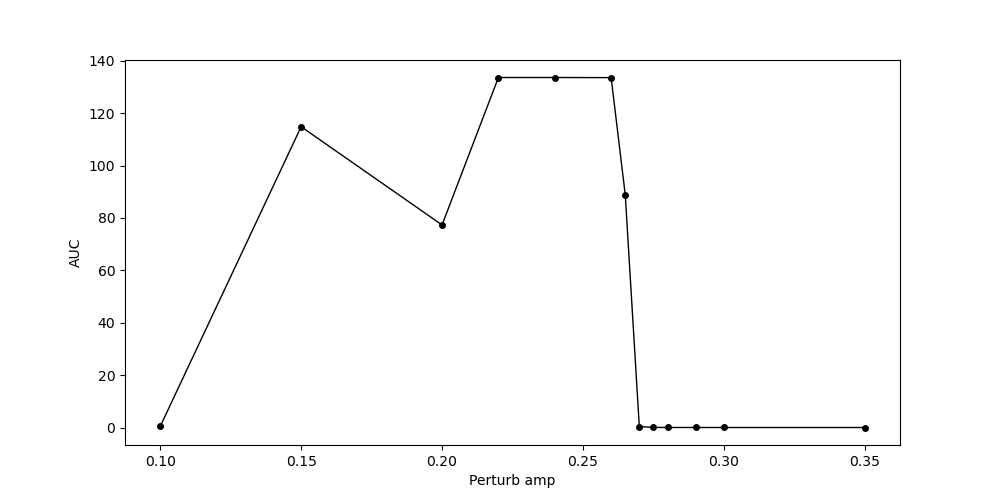
\includegraphics[width=0.9\textwidth]{FNN/fig/temp_abb05_perturbamp_auc_outsigmoid.png} \\
    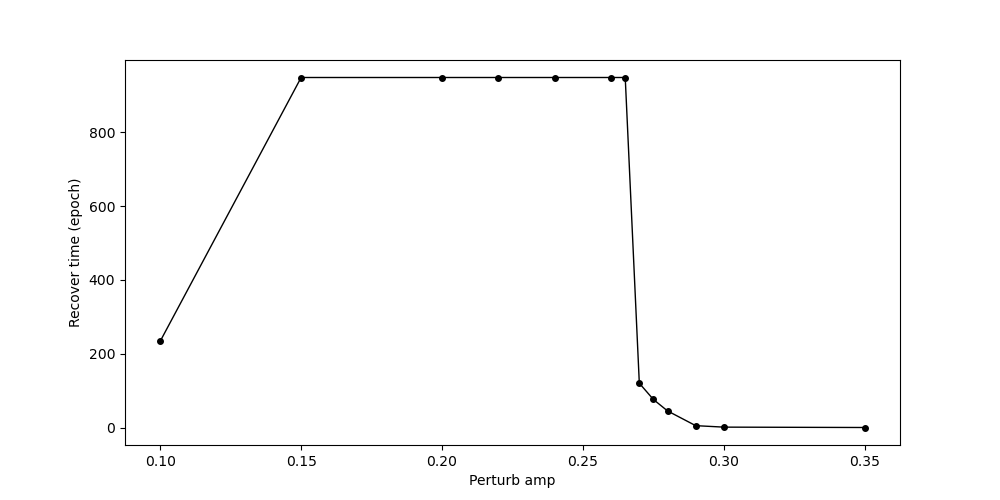
\includegraphics[width=0.9\textwidth]{FNN/fig/temp_abb05_perturbamp_rectime_outsigmoid.png} \\
\end{figure}

More investigation into the details (like under what condition should it converge under perturbation) is needed.

\newpage

%%%%%%%%

\section*{Week 01/22 - 02/20}

\subsection*{Goal}

\noindent
Main Task: Transfer of learning from gains to synapses.

\begin{itemize}
    \item Get the transfer of learning feedforward network work. Try to look at the scale of weights.
    \item Systematically investigate the adaptation to perturbation.
    \item Think of a better way to implement hebbian learning in RNN, especially inhibitory hebbian learning.
\end{itemize}

\noindent
Reading

\begin{itemize}
    \item Bouchard, K. E., Ganguli, S., \& Brainard, M. S. (2015). Role of the site of synaptic competition and the balance of learning forces for Hebbian encoding of probabilistic Markov sequences. Frontiers in Computational Neuroscience, 9.
    \item Rajan, K., \& Abbott, L. F. (2006). Eigenvalue Spectra of Random Matrices for Neural Networks. Physical Review Letters, 97(18), 188104.
    \item Murphy, B. K., \& Miller, K. D. (2009). Balanced Amplification: A New Mechanism of Selective Amplification of Neural Activity Patterns. Neuron, 61(4), 635–648.
    \item Oja, E. (1982). Simplified neuron model as a principal component analyzer. Journal of Mathematical Biology, 15, 267--273.
    \item Hennequin, G., Agnes, E. J., \& Vogels, T. P. (2017). Inhibitory Plasticity: Balance, Control, and Codependence. Annual Review of Neuroscience, 40(1), 557–579.
\end{itemize}

\newpage

\subsection*{Transfer of Learning in Feedforward Network}

We were facing the scaling problem last week that the weights and the outputs have a correct cosine shape but not the correct value. I scrutinized but couldn't find any difference between my code and Swinehart's code. So at last, I tuned and changed the gain and shift of the output node, from gain = 3 and shift = 1 to gain = 6.67 and shift = 1.035 (after all, there is nothing special about 3 and 1). These parameters are selected so that Hebbian learning could converge at the correct value given the input nodes have initial gains and shifts and the output node has target activation.

Below are more training details:
\begin{itemize}
    \item Two layers. 230 Input nodes. 1 Output nodes. Model stucture is shown in Figure 7.
    \item The input nodes have gaussian receptive field for different stimulus value determining the input current $I_i$, and sigmoid activation function $r_i = \frac{1}{1 + e^{-g_i(I_i-s_i)}}$, where initially gain $g_i = 3$ and shift $s_i = 1$. $g_i$ and $s_i$ could be adjusted during training.
    \item The output node is connected to input nodes through weights $w_i$, and has sigmoid activation function $r_o = \frac{1}{1 + e^{-g_o(\sum w_ir_i - s_o)}}$, where gain $g_i = 6.67$ and shift $s_i = 1.035$.
    \item The task is to approximate a cosine function. For the supervisor, we use squared error loss and SGD on gains and shifts of input nodes with learning rate = 0.2.
    \item Hebbian learning is applied to weights, $w_i \rightarrow w_i + \eta r_i r_o$, where $\eta$ gradually increase from 0 until reaching maximum = 0.0001 at 80th epoch. After each update there is also a normalization step to keep all the weights sum to 5.5.
    \item A passive boundary at gains and shifts are applied starting from 20th epoch, that is, in the following epoch the gains and shifts could only be more closed to the initial value than the current epoch.
\end{itemize}

In this way, we make the transfer of learning work.

\begin{figure}[H]
    \centering
    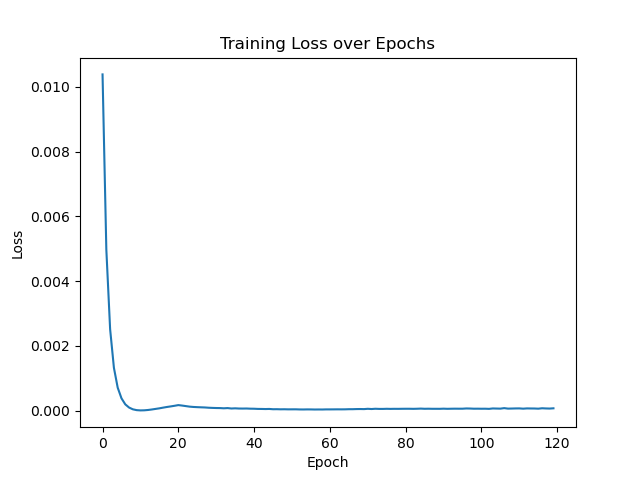
\includegraphics[width=0.6\textwidth]{FNN/fig/0221_abb05_bphebb_loss.png} \\
    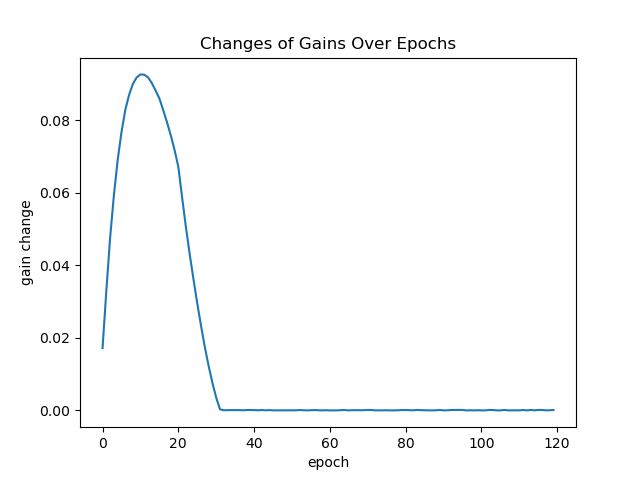
\includegraphics[width=0.6\textwidth]{FNN/fig/0221_abb05_bphebb_gc.png} \\
    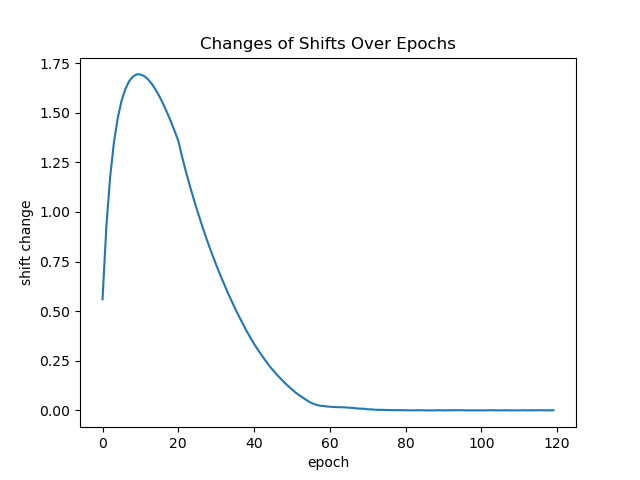
\includegraphics[width=0.6\textwidth]{FNN/fig/0221_abb05_bphebb_sc.png}
\end{figure}

\begin{figure}[H]
    \centering
    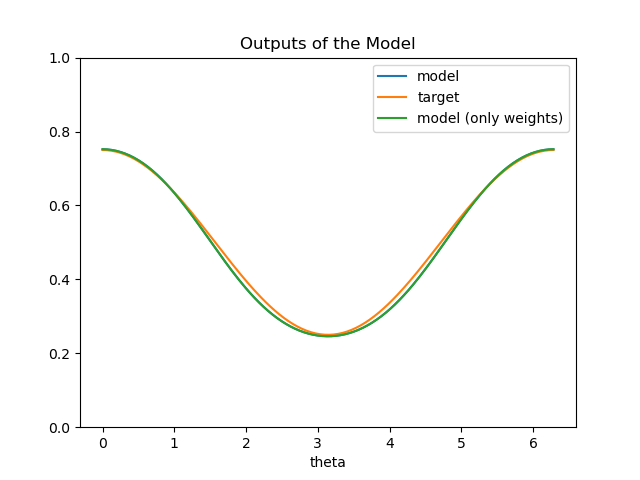
\includegraphics[width=0.8\textwidth]{FNN/fig/0221_abb05_bphebb_output.png} \\
    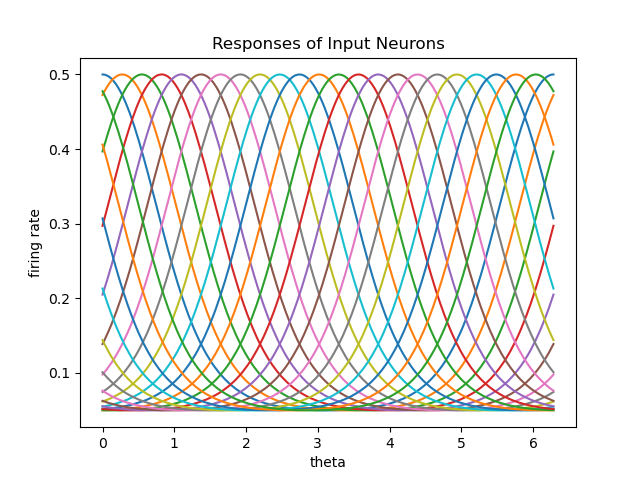
\includegraphics[width=0.8\textwidth]{FNN/fig/0221_abb05_bphebb_rf.png}
\end{figure}

\begin{figure}[H]
    \centering
    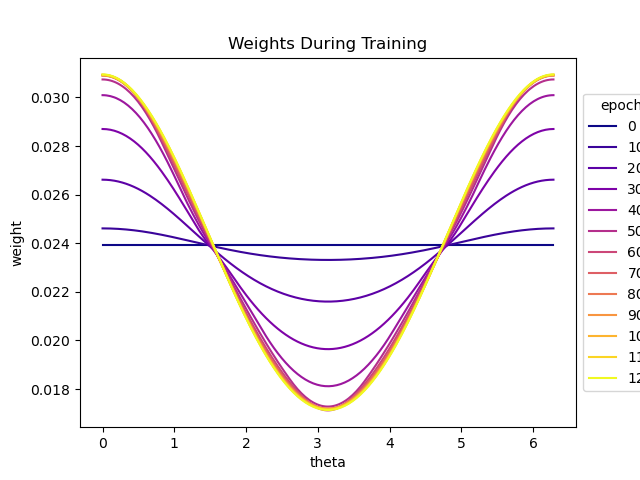
\includegraphics[width=0.8\textwidth]{FNN/fig/0221_abb05_bphebb_timeweights.png} \\
    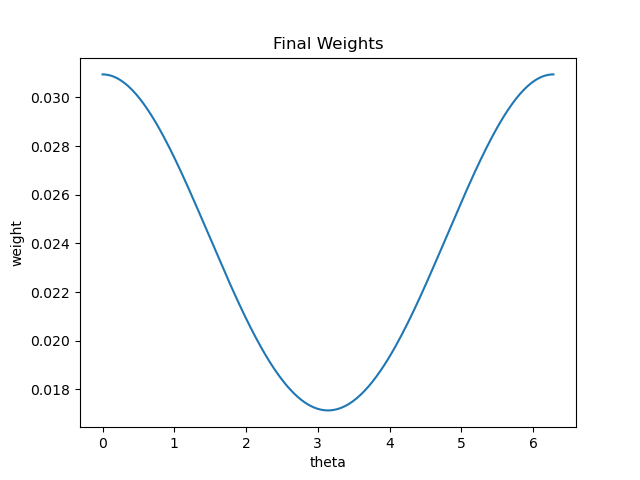
\includegraphics[width=0.8\textwidth]{FNN/fig/0221_abb05_bphebb_finalweights.png}
\end{figure}
\newpage

\subsection*{Perturbation in Feedforward Network}

We want to test whether the network would show some adaptation effect if undergoing a period of persistent perturbation. Using the trained network, we keep the simulation going, add a persistent noise to all input nodes at 50th epoch ($r_i = \frac{1}{1 + e^{-g_i(I_i-s_i) + \epsilon_i}}$, $\epsilon_i \sim N(1,0.001)$), last for certain epochs, and then turn off.

We systemetically control the perturbation lasting to investigate the adaptation effect. To quantify the adaptation, we define two indices to represent the "difficulty" for the network to recover after perturbation: (1) area under the loss curve (AUC) and (2) how many epochs it takes to return to loss $<$ 0.0001. The results show that the longer the perturbation lasts, the harder for a network to recover. And we also observe a tendency of saturation.

\begin{figure}[H]
    \centering
    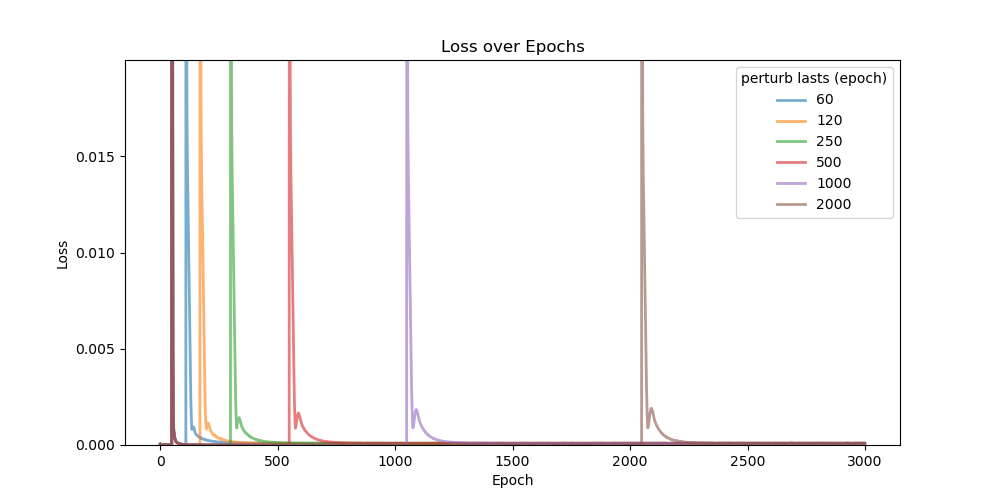
\includegraphics[width=0.8\textwidth]{FNN/fig/0214_abb05_perturb_loss_train.png} \\
    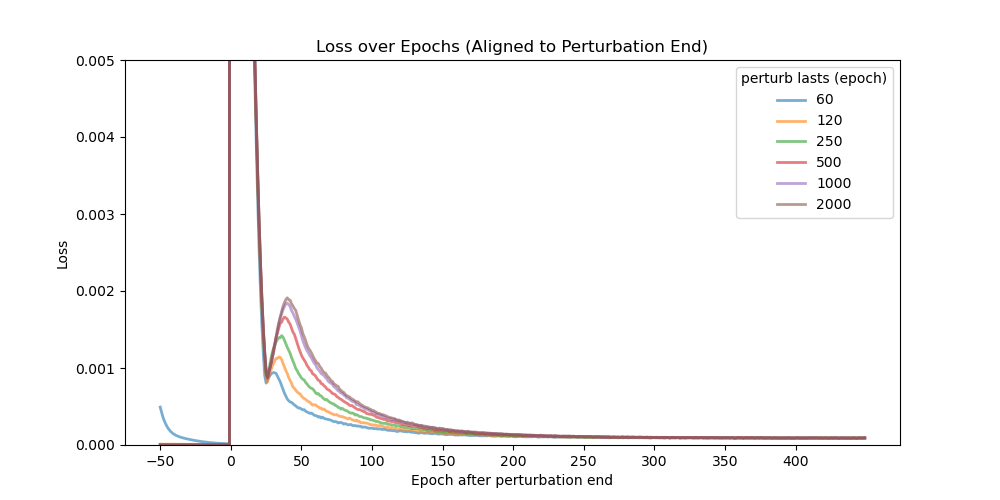
\includegraphics[width=0.8\textwidth]{FNN/fig/0214_abb05_perturb_loss_align.png}
\end{figure}

\begin{figure}[H]
    \centering
    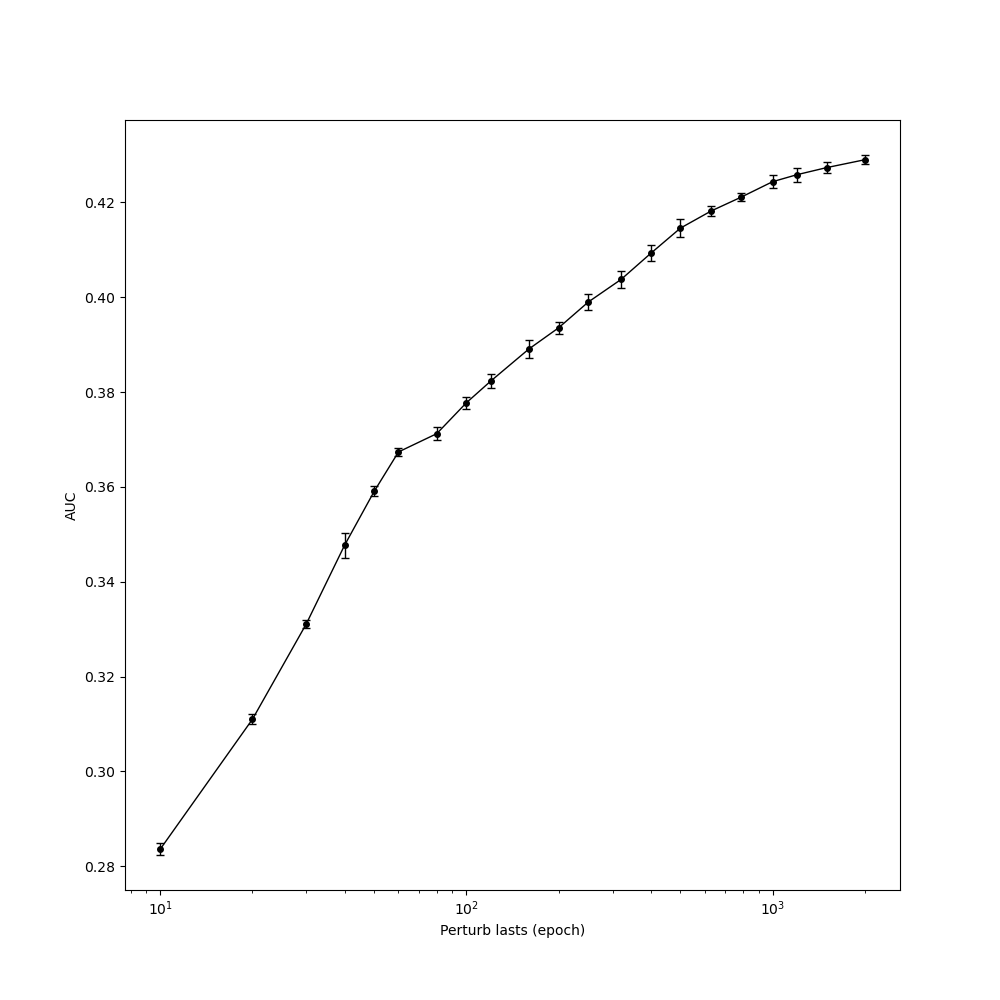
\includegraphics[width=0.7\textwidth]{FNN/fig/0214_abb05_perturb_auc.png} \\
    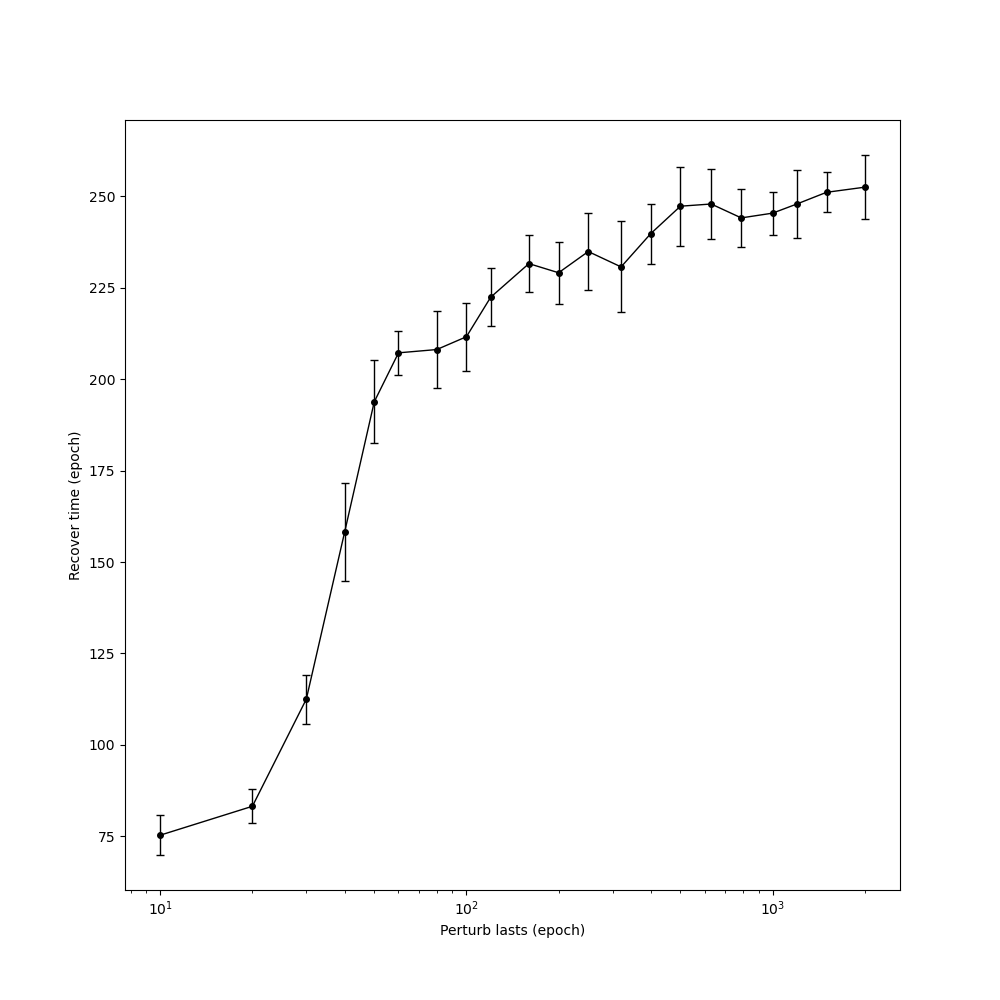
\includegraphics[width=0.7\textwidth]{FNN/fig/0214_abb05_perturb_rectime.png}
\end{figure}

\newpage

We also control the magnitude of perturbation. Here we fix the duration of perturbation as 500 epochs, but change the mean amplitude of noise, i.e., $\epsilon_i \sim N(x, 0.001)$. We find that, if the amplitude of perturbation is too large, the network would fail to learn or reduce its loss under perturbation, and thus recover quickly when the perturbation is turned off. The failure of learning under large perturbation is due to saturation in sigmoid function and thus the gradient vanishes.

\begin{figure}[H]
    \centering
    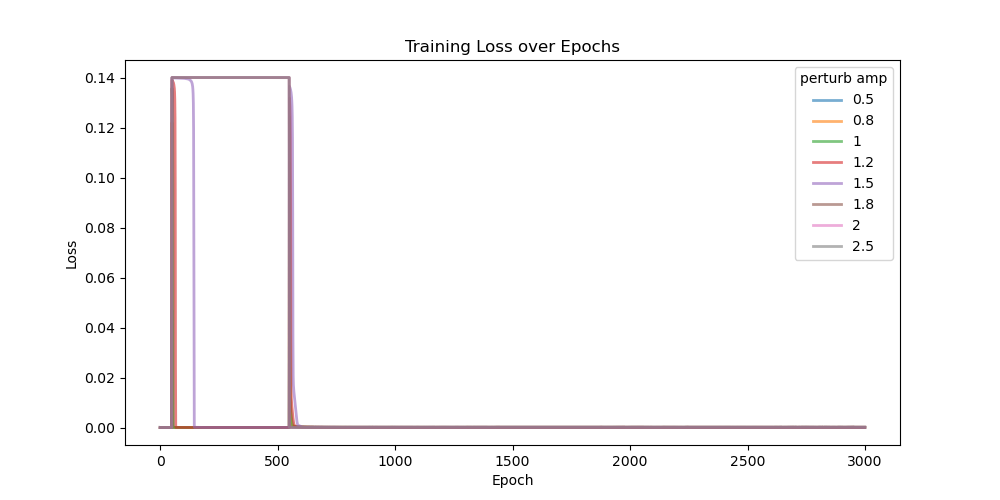
\includegraphics[width=0.8\textwidth]{FNN/fig/0221_abb05_perturbamp_loss.png} \\
    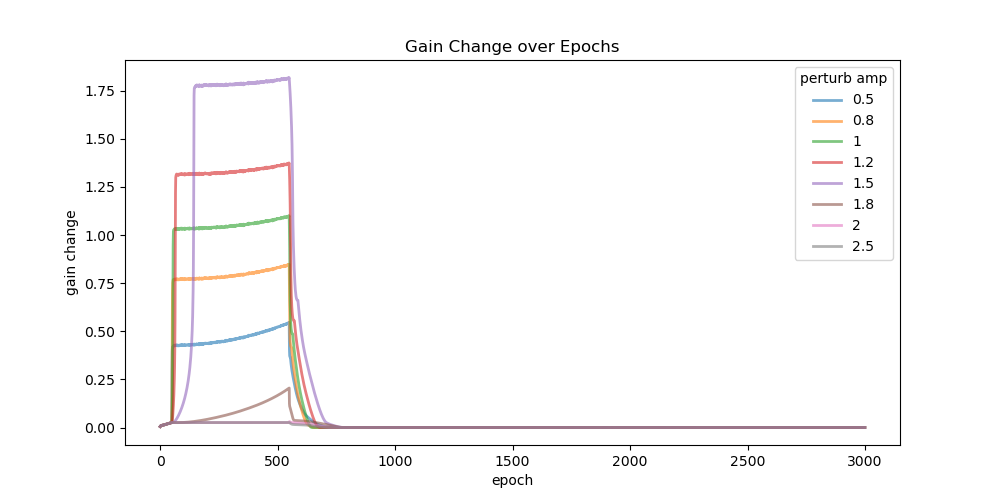
\includegraphics[width=0.8\textwidth]{FNN/fig/0221_abb05_perturbamp_gc.png} \\
    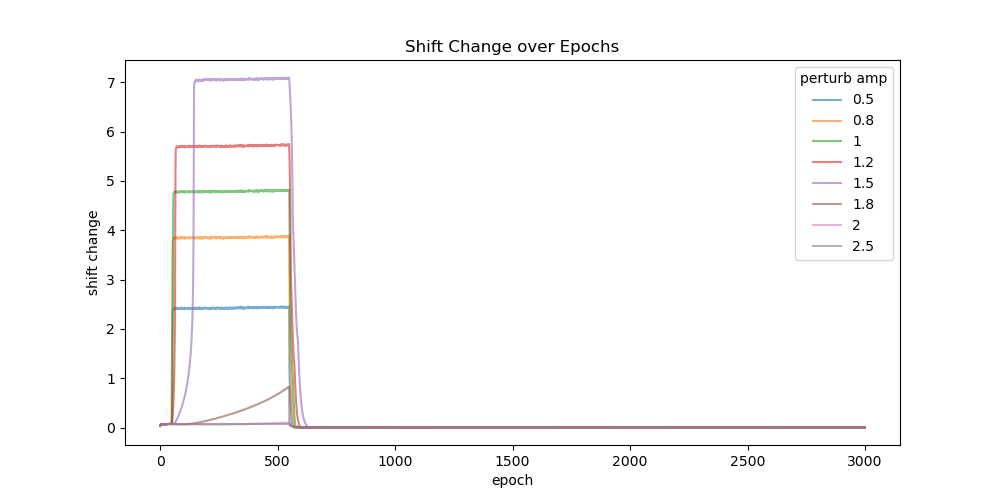
\includegraphics[width=0.8\textwidth]{FNN/fig/0221_abb05_perturbamp_sc.png} \\
\end{figure}

\begin{figure}[H]
    \centering
    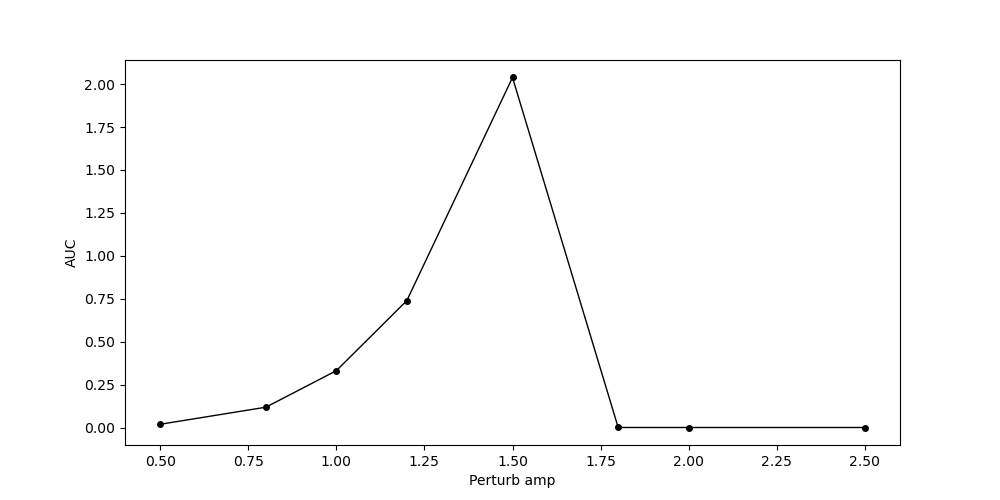
\includegraphics[width=\textwidth]{FNN/fig/0221_abb05_perturbamp_auc.png} \\
    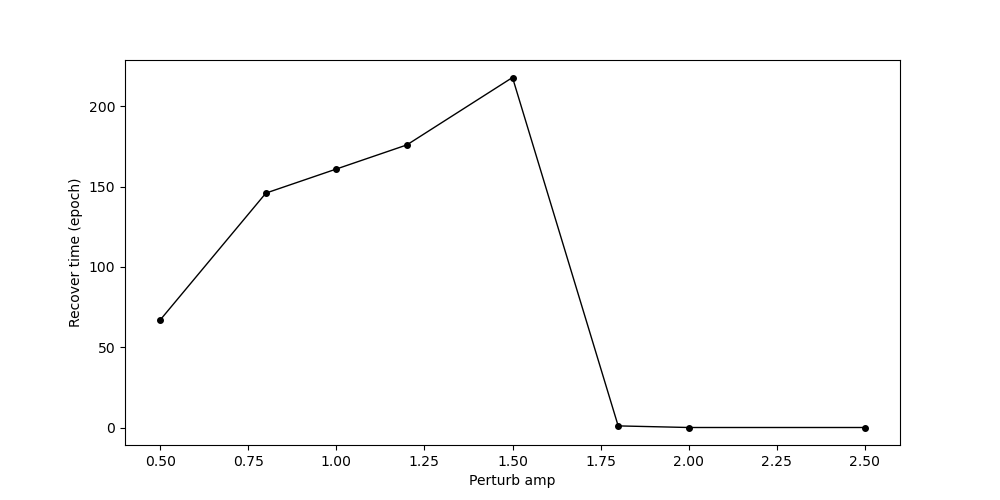
\includegraphics[width=\textwidth]{FNN/fig/0221_abb05_perturbamp_rectime.png} \\
\end{figure}
\newpage

\subsection*{Some Attemps in RNN}

For RNN, I made some attempts in training and modeling. 

\begin{itemize}
    \item Instead of using a input layer matrix to project stimulus value linearly to the recurrent layer, I use a gaussian receptive field for each node in the recurrent layer. There are 32 nodes in recurrent layer, 16 nodes are excitatory and 16 nodes are inhibitory. Each pair of excitatory and inhibitory nodes has the same receptive field, covering the whole range of stimulus value. For the output layer, instead of being random, now I use all 1 (for excitatory nodes) and -1 (for inhibitory nodes).
    \item During training, I use SGD (learning rate = 0.1) to update the gains and shifts in the recurrent layer for each data point in the sine wave. Initial gains are set to 1 and initial shifts are set to 0. If the mean loss of a period of sine wave is less than 0.001 and there have been 1000 periods, hebbian learning would start. Initial weight matrix are set to be uniform, with excitatory weights sum up to 415 and inhibitory weights sum up to 375.
    \item For Hebbian learning I use Hebbian covariance rule for both excitatory neurons and inhibitory neurons. $\Delta w_{ij} = \pm \eta \sigma_i \sigma_j$ (+ for excitatory nodes and - for inhibitory nodes) where $\sigma_i = r_i(t-1) - \bar{r_i}(t-1)$ and $\sigma_j = r_j(t) - \bar{r_j}(t)$ and $\bar{r}$ is the average activation over previous 5 time steps.
    \item After each step of Hebbian learning, there is a normalization performed for each column of weight matrix, to keep the sum constant. For excitatory columns the sum is kept to be 415/16 and for inhibitory columns the sum is kept to be 375/16.
\end{itemize}

The weights now show a interesting shape. But still I might need to look for more plausible inhibitory plasticity. I still reading papers about mathematical analysis of RNN like eigenvalues spectrum and Schur decomposition. Also, it's worth adding weight dependence of synaptic plasticity and difference rate in depression and potentiation.

\newpage

\begin{figure}[H]
    \centering
    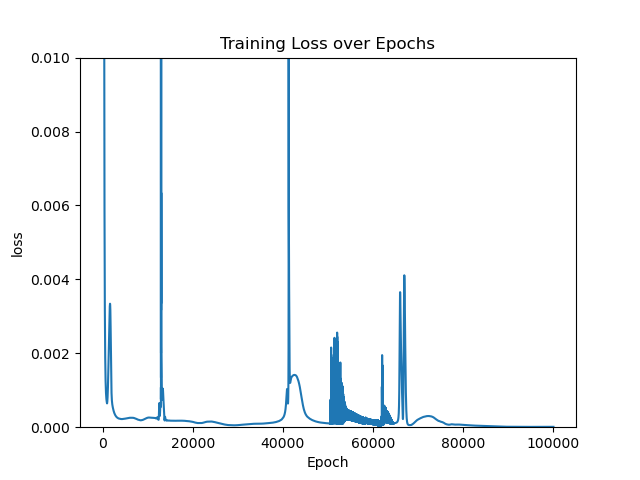
\includegraphics[width=0.6\textwidth]{RNN/ourRNN/analysis/fig/0221_SIN2_bphcppt_loss.png} \\
    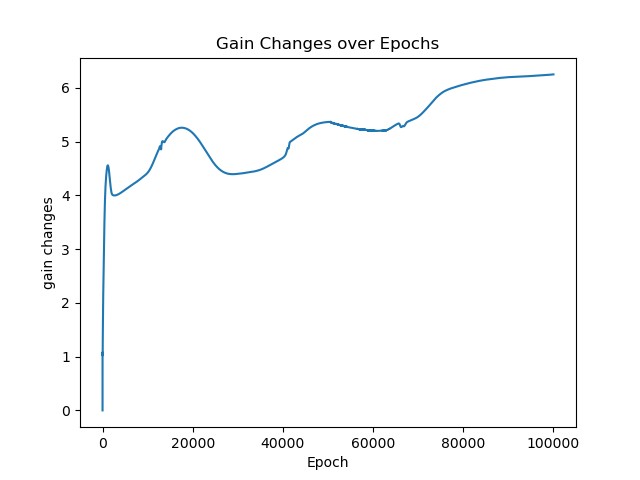
\includegraphics[width=0.6\textwidth]{RNN/ourRNN/analysis/fig/0221_SIN2_bphcppt_gc.png} \\
    \includegraphics[width=0.6\textwidth]{RNN/ourRNN/analysis/fig/0221_SIN2_bphcppt_sc.png} \\
\end{figure}

\begin{figure}[H]
    \centering
    \includegraphics[width=\textwidth]{RNN/ourRNN/analysis/fig/0221_SIN2_bphcppt_output.png} \\
    \includegraphics[width=\textwidth]{RNN/ourRNN/analysis/fig/0221_SIN2_bphcppt_weight_matrix.png}
\end{figure}

\begin{figure}[H]
    \centering
    \includegraphics[width=\textwidth]{RNN/ourRNN/analysis/fig/0221_SIN2_bphcppt_weight_matrix_overtime.png} 
\end{figure}

\newpage

%%%%%%%%%

\section*{Week 11/27 - 01/22}

\subsection*{Goal}

\noindent
Main Task: Transfer of learning from gains to synapses.

\begin{itemize}
    \item Find out how Swinehart and Abbott (2005) manage to do the transfer of learning
    \item Try hard decay on gain modulation magnitude
    \item Try persistent perturbation rather than periodic perturbation
    \item Slowly grow the Hebbian learning rate, avoid abrupt change
    \item On RNN, try inhibitory synaptic plasticity and get the transfer of learning work
\end{itemize}

\noindent
Reading

\begin{itemize}
    \item Vogels, T. P., Sprekeler, H., Zenke, F., Clopath, C., \& Gerstner, W. (2011). Inhibitory Plasticity Balances Excitation and Inhibition in Sensory Pathways and Memory Networks. Science, 334(6062), 1569–1573.
    \item Vogels, T. P., Froemke, R. C., Doyon, N., Gilson, M., Haas, J. S., Liu, R., Maffei, A., Miller, P., Wierenga, C. J., Woodin, M. A., Zenke, F., \& Sprekeler, H. (2013). Inhibitory synaptic plasticity: Spike timing-dependence and putative network function. Frontiers in Neural Circuits, 7.
    \item Rozell, C., Johnson, D., Baraniuk, R., \& Olshausen, B. (2007). Locally Competitive Algorithms for Sparse Approximation. 2007 IEEE International Conference on Image Processing, IV-169-IV–172.
    \item Paul, A., Wagner, S., \& Das, A. (2022). Learning in Feedback-driven Recurrent Spiking Neural Networks using full-FORCE Training (arXiv:2205.13585). arXiv.
    \item Ogawa, S., Fumarola, F., \& Mazzucato, L. (2023). Multitasking via baseline control in recurrent neural networks. Proceedings of the National Academy of Sciences, 120(33), e2304394120.
\end{itemize}

\newpage

\subsection*{Transfer of Learning in Feedforward Network}

% Last week, I demonstrated a way to transfer learning in gains and shifts to weights. However, it is based on switching hebbian learning on and off frequently: only if the loss for a particular data point is small, hebbian learning is performed. I also actively narrow the gains and shifts boundary. It turns out that it does not work well for RNN or adpatation to perturbation.

Ideally, after doing backprop on gains and shifts, the response tuning curves of side neurons would go up and those of middle neurons would go down. Then, when hebbian learning is turning on, the weights of side neurons would get larger update than those of middle nuerons. Plus, the normalization process would keep the sum of the weights as constant, resulting in a cosine-like weights. The changed weights would "exaggerate" the model outputs (e.g., even lower outputs in the middle of the curve). So, to reduce the loss, The next rounds of backprop would flatten the response tuning curves. In theory, this process transfers the learning in gains and shifts to weights. (We don't really need to actively shrink of gains and shifts by putting a shrinking boundaries. In fact, if the shrinkage/flattening goes too fast, hebbian learning could not result in enough curvature in weights.)

\begin{figure}[H]
    \centering
    \includegraphics[width=0.45\textwidth]{FNN/fig/abb05_struc.png}
    \includegraphics[width=0.45\textwidth]{FNN/fig/abb05_paperresult_draw.jpg}
    \\
    \caption{The sturcture and the claimed result in the paper.}
\end{figure}

In practice, the process could not transfer the learning completely, returning the gains and shifts to the initial values. It would converge to a state where the learning is partly in weights and partly in gains and shifts. 

\begin{figure}[H]
    \centering
    \includegraphics[width=0.3\textwidth]{FNN/fig/0122_abb05_bphebb_onlyweights.png}
    \includegraphics[width=0.3\textwidth]{FNN/fig/0122_abb05_bphebb_rf.png}
    \includegraphics[width=0.3\textwidth]{FNN/fig/0122_abb05_bphebb_weights.png}
    \\
    \includegraphics[width=0.3\textwidth]{FNN/fig/0122_abb05_bphebb_loss.png}
    \includegraphics[width=0.3\textwidth]{FNN/fig/0122_abb05_bphebb_gc.png}
    \includegraphics[width=0.3\textwidth]{FNN/fig/0122_abb05_bphebb_sc.png}\\
    \caption{Hebbian learning start after 10 epoches.}
\end{figure}

To understand this, I did an experiment where I keep the gains and shifts unchanged as initial and use backprop to find the "correct" weights. Then I turn on the hebbian learning, but the "correct" weights is not stable. In fact, it would converge to some weights whose loss is high. In other words, the "correct" weights is not a convergence point of hebbian learning.

\begin{figure}[H]
    \centering
    \includegraphics[width=0.45\textwidth]{FNN/fig/0122_abb05_wt_weights.png}
    \includegraphics[width=0.45\textwidth]{FNN/fig/0122_abb05_wtconv_loss.png} \\
    \includegraphics[width=0.45\textwidth]{FNN/fig/0122_abb05_wtconv_weights.png}
    \includegraphics[width=0.45\textwidth]{FNN/fig/0122_abb05_wtconv_output.png}
    \caption{Changes after Hebbian learning on initial gains and correct weights.}
\end{figure}

Mathemetically, the convergence point of hebbian learning should meet some requirements. Say, there are $n$ input nodes and $m$ inputs. For the $i$th input, the activation of input nodes are $a_{i1},\dots,a_{in}$. The target output is $y_i$. Let $w_j$ be the weight from $j$th input nodes to the output node. Denote matrix $A={a_{ij}}$, vector $y=(y_1,\dots,y_n)^T$, vector $w=(w_1,\dots,w_n)^T$. So the "correct" weights should satisfy: $$Aw=y$$
The hebbian update before normalization to the weights would be $A^Ty$. If the weights are to remain the same, the hebbian update should be in the same direction as original weights: $$A^Ty=kw$$
This leads us to $A^TAw=kw$, meaning that only if the "correct" weights are eigenvectors of $A^TA$ could hebbian learning converge.

\subsection*{Perturbation in Feedforward Network}

After the network is trained, I try to add a persistent deviation in neurons' activation after 50 epoches, The perturbation lasts for 1000, 2000, or 5000 epoches. From the losses one could see, the network adapts to the perturbation quickly (with both backprop and hebbian learning), and after the perturbation is turned off, the loss goes up suddenly but gradually goes back to normal.

\begin{figure}[H]
    \centering
    \includegraphics[width=0.45\textwidth]{FNN/fig/0122_abb05_perturb_loss.png} \\
    \includegraphics[width=0.45\textwidth]{FNN/fig/0122_abb05_perturb_gc.png} 
    \includegraphics[width=0.45\textwidth]{FNN/fig/0122_abb05_perturb_sc.png}
    \caption{Perturbation in feedforward netork.}
\end{figure}

\newpage

\subsection*{Transfer of learning in RNN}

I implement the same training paradigm to train the RNN, i.e., first do backprop on gains and shifts and then turn on hebbian learning, to see how much of the learning could be transfered from gains and shifts to weights.

Some details: 32 nodes in recurrent layer; hebbian learning is performed for every timestep; evenly distributed gaussian receptive fields for each neuron; output weight matrix are set to all 1 and -1; one epoch represents 1 period of sinwave with 120 timesteps.

For inhibitory synaptic plasticity, I didn't find a principle applicable for firing rate network. Existing attempts are all based on spike timings. So I just use the same idea as in excitatory synapses: the more they are firing together, the inhibitory synapses are stronger (more negative).

\begin{figure}[H]
    \centering
    \includegraphics[width=0.3\textwidth]{RNN/ourRNN/analysis/fig/0122_SIN2_bphebbpt_output.png}
    \includegraphics[width=0.3\textwidth]{RNN/ourRNN/analysis/fig/0122_SIN2_bphebbpt_activations.png}
    \includegraphics[width=0.3\textwidth]{RNN/ourRNN/analysis/fig/0122_SIN2_bphebbpt_weight_matrix.png}\\
    \includegraphics[width=0.3\textwidth]{RNN/ourRNN/analysis/fig/0122_SIN2_bphebbpt_loss.png}
    \includegraphics[width=0.3\textwidth]{RNN/ourRNN/analysis/fig/0122_SIN2_bphebbpt_gc.png}
    \includegraphics[width=0.3\textwidth]{RNN/ourRNN/analysis/fig/0122_SIN2_bphebbpt_sc.png}\\
    \caption{Hebbian learning start after 1000 epoches.}
\end{figure}

Notice the grid-like weights after hebbian learning. It is quite different from the "correct" weights obtained from backprop on weights.

\begin{figure}[H]
    \centering
    \includegraphics[width=0.45\textwidth]{RNN/ourRNN/analysis/fig/0122_SIN2_wt_weight_matrix.png}
    \caption{Weight matrix after backprop on weights.}
\end{figure}

\subsection*{Perturbation in RNN}

After the network is trained, I try to add a persistent deviation in the input after 50 epoches, The perturbation lasts for 2000, 5000, or 10000 epoches.

\begin{figure}[H]
    \centering
    \includegraphics[width=0.6\textwidth]{RNN/ourRNN/analysis/fig/0122_SIN2_perturb_loss.png} \\
    \includegraphics[width=0.45\textwidth]{RNN/ourRNN/analysis/fig/0122_SIN2_perturb_gc.png} 
    \includegraphics[width=0.45\textwidth]{RNN/ourRNN/analysis/fig/0122_SIN2_perturb_sc.png}
    \caption{Perturbation in RNN.}
\end{figure}

\subsection*{Thoughts}

\begin{itemize}
    \item Hebbian learning may not be able to transfer all the learning from gains and shifts to weights. Hebbian learning is after all unsupervised learning, especially in RNN, how could $n$ nodes instruct $n^2$ weights to learn?
    \item How to change backprop to feedback control is another problem. As our RNN is trained with backprop and it is backprop that reaches a balance with hebbian learning, it is hard for feedback control to reach a similar balance. Primitive attempt reveals that hebbian learning would cause the output drift away under feedback control.
    \item A plausible inhibitory synapses learning rule is yet to find. Maybe we should try on building the spiking neural network?
\end{itemize}

\newpage

%%%%%%%

\section*{Week 11/13 - 11/27}

\subsection*{Goal}

\noindent
Main Task: Adaptative gain modulation and feedback control. Learn the perturbation pattern and gradually transfer the learning to synaptic plasticity.

\begin{itemize}
    \item Predictive feedback control: learn to give a control input in advance to correct the periodic perturbation.
    \item Transfer of learning: using Oja learning to transfer the learning effect from gains to synaptic weights.
\end{itemize}

\noindent
Reading

\begin{itemize}
    \item Bittner, K. C., Milstein, A. D., Grienberger, C., Romani, S., \& Magee, J. C. (2017). Behavioral time scale synaptic plasticity underlies CA1 place fields. Science, 357(6355), 1033–1036.
    \item Bouchard, K. E., Ganguli, S., \& Brainard, M. S. (2015). Role of the site of synaptic competition and the balance of learning forces for Hebbian encoding of probabilistic Markov sequences. Frontiers in Computational Neuroscience, 9.
\end{itemize}

\newpage

\subsection*{Predictive Feedback Control Framework}

One possible framework that is able to predictively give control signal to correct periodic perturbation is to use another neural network with Q-learning.

\begin{figure}[H]
    \centering
    \includegraphics[width=0.8\textwidth]{RNN/ourRNN/analysis/fig/qlearn_struc.jpg}
\end{figure}

Let the state at time $t$ be $x_t$. Given $x_t$, An action $a_t$ (i.e., control signal) could drive the state $x_t$ to some $x_{t+1}$. We define the reward $r_{t+1}$ associate with $x_{t+1}$ as the negative of the distance between the output and the target.

We define the estimated state-action value as $Q(x_t, a_t)$. The goal is to learn the $Q$ function so that it can correctly estimate the future rewards when exert an action $a_t$ at the state $x_t$. Once we have a good $Q$, given $x_t$, we just need to choose $a_t$ that maximize $Q(x_t, a_t)$ as our control signal.

To approximate the function $Q$, we may need to use another simple neural network (since there are infinitely many states and actions), so that $Q(s,a) \approx Q(s,a;\theta)$. The loss function would be 
$$ L = E \left[ \left( r_{t+1} + \gamma \max_{a} Q(s_{t+1},a; \theta) - Q(s_t, a_t; \theta) \right)^2 \right] $$
To simplify, we could assume $\max_{a} Q(s_{t+1}, a; \theta) = 0$, so $ L = E \left[ \left( r_{t+1} - Q(s_t, a_t; \theta) \right)^2 \right] $. 

But training this neural network requires back propagation. Also it would substitute LQR once it is fully functioning.

\newpage

\subsection*{Transfer of Learning}

To explore transfer of learning, I first explore the gains and weights during the initial training (no perturbation). However, it seems that gains are not converging. (By reflection it might be because of Adam optimizer. Shall try SGD later.) Gain change represents the distance between current gains and initial gains. Weight sum represents sum of weights.

I also try to replicate the simple neural network in Swinehart and Abbott (2005), using SGD and Hebbian learning. But it seems that the learning in gains doesn't completely transfer into the weights.

\newpage

%%%%%%%%

\section*{Week 10/31 - 11/13}

\subsection*{Goal}

\noindent
Main Task: Feedback control in non-linear system under periodic perturbation.

\begin{itemize}
    \item Get extended kalman filter and non-linear LQR to make the gain modulation RNN work under feedback control
    \item Add instant noise onto sustained noise
    \item Test Hebbian learning under noise
\end{itemize}

\noindent
Reading

\begin{itemize}
    \item \url{https://en.wikipedia.org/wiki/Extended_Kalman_filter}
    \item Li, W., \& Todorov, E. (2004). Iterative linear quadratic regulator design for nonlinear biological movement systems. Proceedings of the First International Conference on Informatics in Control, Automation and Robotics, 222–229.
    \item Sober, S. J., \& Brainard, M. S. (2009). Adult birdsong is actively maintained by error correction. Nature Neuroscience, 12(7), 927–931.
    \item Warren, T. L., Tumer, E. C., Charlesworth, J. D., \& Brainard, M. S. (2011). Mechanisms and time course of vocal learning and consolidation in the adult songbird. Journal of Neurophysiology, 106(4), 1806–1821.
    \item Sober, S. J., \& Brainard, M. S. (2012). Vocal learning is constrained by the statistics of sensorimotor experience. Proceedings of the National Academy of Sciences, 109(51), 21099–21103.
\end{itemize}

\newpage

\subsection*{Model}
\begin{itemize}
    \item Structure: 1 input layer (1D input), 1 recurrently-connected hidden layer (128 nodes) where 50\% are excitatory neurons (obeying Dale's law), 1 output layer (1D output).

    \item Activation function: sigmoid function $f(y, u) = \frac{1}{1 + e^{-(g + u)(y - s)}}$, where $y$ is the input activation, $u$ is the control input, $g$ is the gain, and $s$ is the shift. 
    
    \item Equations: 
    \begin{eqnarray}
    \nonumber
    x_{t+1} = f(Wx_t + I_{t}, u_{t}) + w_d \\
    \nonumber
    y_t = Cx_{t} + w_n
    \end{eqnarray}
    
    $x_t$ is the activation, $I_t$ is the input after input layer, $u_t$ is the control input, $w_d$ is the Gaussian processing noise following $N(0,W_d)$, $w_n$ is the Gaussian measurement noise following $N(0,W_n)$, $W$ is the weight matrix, $C$ is set to be identity matrix.

    \item Training: Only SGD on gains and shifts. The same model as Week 10/1-10/16.

    \item Feedback control: extended Kalman filter and nonlinear LQR. The basic idea is to use the Jacobian matrix of $f$ at given $x_t$ to approximate linear system.
    
    \item For both SIN and MG, $Q = 10I$, $R = 0.01I$, $W_d = 0.001I$, $W_n = 0.001I$.

\end{itemize}

\newpage

\subsection*{Periodic Perturbation}

\begin{figure}[H]
    \centering
    \includegraphics[width=\textwidth]{RNN/ourRNN/analysis/fig/1113_SIN_lqg.png}
    \caption{SIN, RNN and LQG on gains under periodic noise, without onging hebbian learning.}
\end{figure}

\begin{figure}[H]
    \centering
    \includegraphics[width=\textwidth]{RNN/ourRNN/analysis/fig/1113_MG_lqg.png}
    \caption{MG, RNN and LQG on gains under periodic noise, without onging hebbian learning.}
\end{figure}

\newpage

\subsection*{SIN with Onging Oja Learning}

Oja learning can't ensure a steady performance without noise. The effect of Oja learning is closely related with $\alpha$. When $\alpha$ is large, the regulation term is large, the sum of weights go down making the output go up. When $\alpha$ is small, the regulation term is small, the sum of weights go up making the output go down. Need to investigate how hebbian-like learning could perform stable performance under no error and compensate performance when error occurs.

\newpage

%%%%%%%%

\section*{Week 10/16 - 10/31}

\subsection*{Goal}

\noindent
Main Task: Feedback control to Linear RNN, and test the performance under noise.

\begin{itemize}
    \item Add gaussian noise
    \item Add Kalma filter and LQR control signal
\end{itemize}

\noindent
Reading

\begin{itemize}
    \item Charles, A. S., Balavoine, A., \& Rozell, C. J. (2016). Dynamic Filtering of Time-Varying Sparse Signals via $\ell _1$ Minimization. IEEE Transactions on Signal Processing, 64(21), 5644–5656.
    \item Rubin, R., Abbott, L. F., \& Sompolinsky, H. (2017). Balanced excitation and inhibition are required for high-capacity, noise-robust neuronal selectivity. Proceedings of the National Academy of Sciences, 114(44).
    \item Zhang, Z., \& Fujisaki, Y. (2023). Sparse Feedback Controller: From Open-loop Solution to Closed-loop Realization (arXiv:2303.15175). arXiv.
\end{itemize}

\newpage

\subsection*{Model}
\begin{itemize}
    \item Structure: 1 input layer (1D input), 1 recurrently-connected hidden layer (32 nodes) where 50\% are excitatory neurons (obeying Dale's law), 1 output layer (1D output). 

    \item Activation function: for now $y=x$ to make it a simple linear system.
    
    \item Equations: 
    \begin{eqnarray}
    \nonumber
    \dot{x_t} = (W-I)x_t + I_{t} + u_{t} + w_d \\
    \nonumber
    y_t = Cx_{t} + w_n
    \end{eqnarray}
    
    \item $x_t$ is the activation, $I_t$ is the input after input layer, $u_t$ is the control input, $w_d$ is the Gaussian processing noise following $N(0,W_d)$, $w_n$ is the Gaussian measurement noise following $N(0,W_n)$, $W$ is the weight matrix, $C$ is set to be identity matrix.

    \item In the absense of control input and noise, use backpropagation to train the weight matrix $W$ so that $x_t$ gives ideal outputs after output layer. We refer to such $x_t$ as reference activations $r_t$.

    \item Kalman filter: $\dot{\hat{x}_t} = (W-I)\hat{x}_t + I_{t} + u_{t} + K_f(y_t - C\hat{x}_t)$.
    
    \item LQR: $u_t = -K(\hat{x}_t - r_t)$, to minimize $\int x^TQx + u^TRu \,dt$.

    \item For SIN, $Q = I$, $R = 0.01I$, $W_d = 0.01I$, $W_n = 0.001I$. For MG, $Q = I$, $R = 0.1I$, $W_d = 0.001I$, $W_n = 0.0001I$. These choices, as well as the number of nodes, may influence convergence.

\end{itemize}

% structure plot!
\begin{figure}[H]
    \centering
    \includegraphics[width=0.9\textwidth]{RNN/baseline_linear/fig/lqg_structure.jpg}
\end{figure}

\subsection*{Persistent and Instant Perturbation}

\begin{figure}[H]
    \centering
    \includegraphics[width=\textwidth]{RNN/baseline_linear/fig/SIN_lin_noise.png}
    \caption{SIN, linear RNN and LQG under perturbation, without onging hebbian learning.}
\end{figure}

\begin{figure}[H]
    \centering
    \includegraphics[width=\textwidth]{RNN/baseline_linear/fig/MG_lin_noise.png}
    \caption{MG, linear RNN and LQG under perturbation, without onging hebbian learning.}
\end{figure}

\newpage

%%%%%%%

\section*{Week 10/1 - 10/16}

\subsection*{Goal}

\noindent
Main Task: Establish a basic recurrent neural network!

\begin{itemize}
    \item Get the code from Ankit
    \item Change the acitivation function to sigmoid, and change the synaptic modulation to gain modulation using back-propagation
    \item Simulate sin wave
    \item Simulate Mackey-Glass equation
    \item Obey Dale law
\end{itemize}

\noindent
Reading

\begin{itemize}
    \item Sussillo, D., \& Abbott, L. F. (2009). Generating Coherent Patterns of Activity from Chaotic Neural Networks. Neuron, 63(4), 544–557. \url{https://doi.org/10.1016/j.neuron.2009.07.018}
    \item Nicola, W., \& Clopath, C. (2017). Supervised learning in spiking neural networks with FORCE training. Nature Communications, 8(1), 2208. \url{https://doi.org/10.1038/s41467-017-01827-3}
    \item Maass, W., Natschläger, T., \& Markram, H. (2002). Real-Time Computing Without Stable States: A New Framework for Neural Computation Based on Perturbations. Neural Computation, 14(11), 2531–2560. \url{https://doi.org/10.1162/089976602760407955}
    \item \url{https://en.wikipedia.org/wiki/Reservoir_computing}
\end{itemize}

\newpage

\subsection*{Model}
\begin{itemize}
    \item Structure: 1 input layer (1D input), 1 recurrently-connected hidden layer (128 nodes), 1 output layer (1D output).
    \item Activation function: sigmoid function $r_i = \frac{1}{1 + e^{-g_i(I_i-s_i)}}$, where $I_i$ is the input, $r_i$ is the output, $g_i$ is the gain, $s_i$ is the shift. 
    \item Initialization: input weights, internal weights, output weights, gains, and shifts are randomly initialized using Gaussian distribution. Initial activations are initialized as 0.
    \item Dale's law: specify a proportion of neurons to be excitatory (here 50\%) and others to be inhibitory. excitatory neurons can only have positive weights and inhibitory neurons can only have negative weights.
    \item Tasks:
    \begin{enumerate}
        \item Predict sine wave: $f(t)=sin(at)$, $a=\frac{1}{60\pi}$. Input $f(t)$, train RNN to predict $f(t+1)$.
        \item Predict Mackey-Glass equation: $\frac{d}{dt}g(t)=\frac{\beta_0 g(t-\tau)}{1+g(t-\tau)^n}-\gamma g(t)$, 
        
        $\gamma=0.1, \beta_0=0.2, n=10, \tau=20$. Input $g(t)$, train RNN to predict $g(t+1)$.
    \end{enumerate}
    \item Training: 
    \begin{enumerate}
        \item Gradient descent to update gains and shifts only (SGD optimizer in PyTorch, learning rate=$0.2$).
        % \item Gradient descent on gains and shifts + basic Hebbian learning to update the internal weights ($w_{ij} \rightarrow w_{ij} + \eta r_i r_j$, normalize, $\eta=0.01$ with expnential decay).
        \item Gradient descent on gains and shifts + Oja's learning rule to update the internal weights ($w_{ij} \rightarrow w_{ij} + \eta (r_i r_j - \alpha r_j^2 w_{ij})$, only on weights from excitatory neuron, $\alpha = \sqrt{128}$, $\eta=0.01$ with expnential decay).
    \end{enumerate}


\end{itemize}

\subsection*{SGD on Gains and Shifts Only}

\begin{figure}[H]
    \centering
    \includegraphics[width=\textwidth]{RNN/ourRNN/analysis/fig/1016_SIN_bpgain_output.png}\\
    \includegraphics[width=\textwidth]{RNN/ourRNN/analysis/fig/1016_SIN_bpgain_loss.png}
    \caption{SIN, SGD only.}
\end{figure}

\begin{figure}[H]
    \centering
    \includegraphics[width=\textwidth]{RNN/ourRNN/analysis/fig/1016_MG_bpgain_output.png}
    \includegraphics[width=\textwidth]{RNN/ourRNN/analysis/fig/1016_MG_bpgain_loss.png}
    \caption{MG, SGD only.}
\end{figure}

Training the RNN with gain modulation while keeping the input matrix, internal matrix, and output matrix as random could approximate sine wave and Mackey-Glass equation, and in the meanwhile obeying the Dale's law.

\subsection*{SGD on Gains and Shifts with Oja's Learning}

For Oja's learning plus gradient descent, it only works when it is with Adam optimizer, not the normal SGD optimizer.

\end{document}